%% Template para dissertação/tese na classe UFPEthesis
%% versão 0.9.2
%% (c) 2005 Paulo G. S. Fonseca
%% www.cin.ufpe.br/~paguso/ufpethesis

%% Carrega a classe ufpethesis
%% Opções: * Idiomas
%%           pt   - português (padrão)
%%           en   - inglês
%%         * Tipo do Texto
%%           bsc  - para monografias de graduação
%%           msc  - para dissertações de mestrado (padrão)
%%           qual - exame de qualificação doutorado
%%           prop - proposta de tese doutorado
%%           phd  - para teses de doutorado
%%         * Mídia
%%           scr  - para versão eletrônica (PDF) / consulte o guia do usuario
%%         * Estilo
%%           classic - estilo original à la TAOCP
%%           modern  - estilo à la CUP (padrão)
%%           ugly    - formato da UFPE com parte pré-textual no formato ABNT
%%         * Paginação
%%           oneside - para impressão em face única
%%           twoside - para impressão em frente e verso (padrão)
\documentclass[bsc, pt, oneside]{ufpethesis}

%% Preâmbulo:
%% coloque aqui o seu preâmbulo LaTeX, i.e., declaração de pacotes,
%% (re)definições de macros, medidas, etc.

%% Identificação:

% Universidade
% e.g. \university{Universidade de Campinas}
% Na UFPE, comente a linha a seguir
\university{Universidade Federal de Pernambuco}

% Modifique o comando \universitylogo para alterar o logo da universidade
% e.g.
% \renewcommand{\universitylogo}{\includegraphics{newlogo.pdf}}

% Endereço (cidade)
% e.g. \address{Campinas}
% Na UFPE, comente a linha a seguir
\address{Recife}

% Instituto ou Centro Acadêmico
% e.g. \institute{Centro de Ciências Exatas e da Natureza}
% Comente se não se aplicar
\institute{Centro de Informática}

% Departamento acadêmico
% e.g. \department{Departamento de Informática}
% Comente se não se aplicar
%\department{NOME DO DEPARTAMENTO}

% Programa de pós-graduação
% e.g. \program{Pós-graduação em Ciência da Computação}
\program{Graduação em Engenharia da Computação}

% Área de titulação
% e.g. \majorfield{Ciência da Computação}
\majorfield{Engenharia da Computação}

% Título da dissertação/tese
% e.g. \title{Sobre a conjectura $P=NP$}
\title{Protocolo baseado em LoRa para Sistemas IoT de longas distâncias}

% Data da defesa
% e.g. \date{19 de fevereiro de 2003}
\date{XX de Abril de 2023}

% Autor
% e.g. \author{José da Silva}
\author{Matheus Ferreira Bernardo de Souza}

% Orientador(a)
% Opção: [f] - para orientador do sexo feminino
% e.g. \adviser[f]{Profa. Dra. Maria Santos}
\adviser[f]{Profa. Edna Natividade da Silva Barros}

% Orientador(a)
% Opção: [f] - para orientador do sexo feminino
% e.g. \coadviser{Prof. Dr. Pedro Pedreira}
% Comente se não se aplicar
% \coadviser{NOME DO(DA) CO-ORIENTADOR(A)}

%% Inicio do documento
\begin{document}

%%
%% Parte pré-textual
%%
\frontmatter

% Folha de rosto
% Comente para ocultar
\frontpage

% Portada (apresentação)
% Comente para ocultar
\presentationpage

% Dedicatória
% Comente para ocultar
\begin{dedicatory}
A uma sociedade justa para todos.
\end{dedicatory}

% Agradecimentos
\acknowledgements

Primeiramente eu gostaria de agradecer a Deus por se fazer sempre presente
na minha vida e na vida dos que mais amo. Por meio da ciência consegui enxergar
o mundo, e por meio da fé consegui enxergar além.

Gostaria de agradecer todas as comunidades acadêmicas e comunidades livres.
Onde cheguei e onde irei chegar será sempre graças a ajuda de muitos, uns
que já se foram, uns que estão entre nós. Logo deixo aqui minha gratidão
a todos que se dedicam a uma sociedade aberta para todos.

Agradeço a Mariana de Carvalho Freire por compor a parte mais fundamental
da minha existência. Você é a definição do tudo, minha maior inspiração,
meu maior objetivo. A sua genialidade me ensinou a sabedoria mais
importante, o sentido da vida. Obrigado por me mostrar que existimos
para o amor.

Aos meus pais, Wellington e Sandra, vocês foram o começo de tudo, vocês
que plantaram a semente e dedicaram suas vidas a cultiva-lá na seca e
na tempestade, sempre com fé de que apesar de tudo ela cresceria bem.
Vocês estarão sempre imortalizados em mim e nas sementes que eu plantar.
Serie sempre grato a Deus por ser o filho do amor de vocês.

Aos professores e professoras, quero agradecer primeiramente a Profa. Edna
Barros. A senhora é uma inspiração para mim, lhe admiro e sou muito grato
por todo o suporte e dedicação que a senhora incondicionalmente fornece aos
alunos da universidade. Quero agradecer também a Carlos Mello, Odilon Maroja,
Daniel da Cunha, Divanilson Campelo, Patricia Tedesco, Adriano Sarmento
e Sergio Cavalcanti. Vocês antes de tudo são amigos e conselheiros, agradeço
por compartilharem comigo seus conhecimentos, serão sempre referências de
seres humanos para mim.

Aos amigos e amigas, quero agradecer a Gabriel Monteiro e Joanna Amarante
por terem me ensinado o companheirismo confortante de uma amizade, e ao 
Vitor Eiji por manter esse sentimento. Para o alívio de todos os momentos
um agradecimento especial a Gabriel Mendes, Luiz Braga, Leonardo Barontini,
Katsuya Okubo, Diego Floriano, Felipe Lopes, João Tessuto, Mateus Umbelino,
Pedro Henrique, Ruan Ascariz, Igor Moura, Rodrigo Valença, Gabriela Medeiros,
Rafael Vasconcelos, Thiago Barros, Nathalia Lima, Ladson Gomes, Beatriz Alves
e Marcos Monteiro.

Por fim eu quero agradecer a você, leitor. Que meu trabalho seja para você
uma inspiração assim como outros foram para mim.

% Epígrafe
% Comente para ocultar
% e.g.
%  \begin{epigraph}[Tarde, 1919]{Olavo Bilac}
%  Última flor do Lácio, inculta e bela,\\
%  És, a um tempo, esplendor e sepultura;\\
%  Ouro nativo, que, na ganga impura,\\
%  A bruta mina entre os cascalhos vela.
%  \end{epigraph}
\begin{epigraph}{Mano Brown}
"Lágrimas\\
Molham a medalha de um vencedor,\\
Chora agora ri depois, aí, Jesus chorou."
\end{epigraph}

% Resumo em Português
\resumo
Com o crescimento de aplicações de Big Data e Aprendizagem de Máquina em
áreas como Smart Cities, Smart Farming e Healthcare, a Internet das Coisas
tem o papel fundamental de viabilizadora desses projetos, o que intensifica a
indústria IoT a se manter em constante pesquisa de tecnologias como a LPWAN,
que permite o espalhamento de dispositivos inteligentes em
grandes áreas urbanas e rurais. Dentre elas a LoRa vem ganhando
destaque por suas características atrativas para um sistema IoT de longas distâncias. 
Entretanto a tecnologia LoRa não fornece ao desenvolvedor o suporte de uma rede dos 
dispositivos do seu sistema. Dessa forma, esse trabalho propõem
um protocolo baseado em LoRa para fornecer suporte de rede ao desenvolvedor de
Sistemas IoT.
\begin{keywords}
Sistemas Embarcados, Internet of Things, Low Power Wide Area Network, LoRa, Protocolo de Rede
\end{keywords}

% Resumo em Inglês
\abstract
With the growth of Big Data and Machine Learning applications in fields such as
Smart Cities, Smart Farming and Healthcare, the Internet of Things plays a key
role in facilitating these projects, which intensifies the IoT industry to keep
constantly researching technologies like LPWAN, that allows the scattering of
smart devices in large urban and rural areas. Among then LoRa is standing out
for its attractive features for long-distance IoT systems. However LoRa technology
does not provide a network support to the IoT system developer. In this way, this
thesis proposes a LoRa-based network protocol to provide network support to the
IoT system developer.
\begin{keywords}
Embedded Systems, Internet of Things, Low Power Wide Area Network, LoRa, Network Protocol
\end{keywords}

% Sumário
% Comente para ocultar
\tableofcontents

% Lista de figuras
% Comente para ocultar
\listoffigures

% Lista de tabelas
% Comente para ocultar
\listoftables

%%
%% Parte textual
%%
\mainmatter

% É aconselhável criar cada capítulo em um arquivo à parte, digamos
% "capitulo1.tex", "capitulo2.tex", ... "capituloN.tex" e depois
% incluí-los com:
% \include{capitulo1}
% \include{capitulo2}
% ...
% \include{capituloN}
\chapter{Introdução}

\section{Motivação}

A ascensão da Internet das Coisas (IoT) introduziu aos mais diferentes tipos de objetos
físicos o acesso à internet. Esses objetos, às vezes imperceptíveis no nosso dia a dia,
gerando agora um grande fluxo coletivo de dados em tempo real, que em conjunto às 
tecnologias de Aprendizagem de Maquina (ML) \cite{8001570}, tornou possível aplicações
cada vez mais independentes e inteligentes em diversas áreas como agricultura,
transporte, saúde, entre outras \cite{8883163}\cite{8358540}\cite{7474197}.

Além de suas características físicas, os objetos possuem sistemas eletrônicos embutidos, 
comumente conhecidos como sistemas embarcados. Esses sistemas são baseados em 
microcontroladores com sensores e/ou atuadores. Eles possuem poder computacional, 
conetividade, e energia limitados se
comparados aos dispositivos mais comuns, como smartfones e computadores. Devido a tais 
limitações, a indústria IoT impulsiona pesquisas que viabilizem a construção 
de sistemas inteligentes nos mais restritos cenários \cite{9221219}.

Nos últimos anos, tecnologias como LPWAN (Low Power Wide Area Network) tem tornado
realidade sistemas IoT com objetos 
distribuídos num grande espaço geográfico por oferecerem baixo consumo energético e 
conectividade a longas distâncias \cite{7815384}. Dentre essas tecnologias como
Sigfox e NB-IoT, LoRa (Longe Range) tem ganhado destaque entre elas por sua conectividade 
a distâncias quilométricas, bidirecionalidade, baixo consumo, alta capacidade de nós na 
rede, e por operar na faixa de frequência ISM (Industrial Scientific and Medical),
de livre licença para uso em diversos países \cite{9230597}.

Porém, de maneira simples, LoRa pode ser considerada tanto uma modulação de rádio 
frequência como uma camada física de transmissão de dados, algo que não garante ao 
desenvolvedor IoT um suporte de rede entre os nós e outras aplicações \cite{8474715}.
Com isso, na indústria se propõem diferentes protocolos a serem implementados por cima
da camada física da LoRa que estabelecem uma topologia de rede para o sistema.
Dentre os protocolos, o mais difundido atualmente é o LoRaWAN, um protocolo aberto 
proposto pela LoRa Alliance \cite{8767242}.

A arquitetura LoRaWAN, apesar de apresentar uma solução para o estabelecimento
de rede do sistema IoT, apresenta limitações como presença de nós
desconectados da rede em sistemas com poucos \textit{gateways} de cobertura e
falta de comunicação direta entre os nós \cite{8767242}. 
Tais limitações podem dificultar alguns tipos de sistemas IoT de longas 
distâncias, e dessa maneira ainda se fazem válidas as pesquisas e propostas de 
protocolos baseados em LoRa \cite{8767242}\cite{NAKAMURA2022257}.

\section{Objetivos}

O objetivo \textbf{geral} desse trabalho é propor, documentar e implementar um
protocolo de rede baseado em LoRa que forneça ao desenvolvedor de sistemas IoT
o suporte de rede para seus dispositivos inteligentes usando LoRa.

São objetivos \textbf{específicos} deste projeto:
\begin{itemize}
    \item Criação de documentação e diagramas sobre o protocolo proposto;
	\item Implementação do protocolo em forma de biblioteca;
	\item Execução de testes em dispositivos embarcados para validação do protocolo proposto;
	\item Avaliação dos resultados obtidos.
\end{itemize}

\section{Estrutura do Trabalho}

Neste capítulo são apresentados a motivação desse trabalho assim como o detalhamento dos
objetivos a serem alcançados, e a estruturação escolhida para o documento. Os próximos
capítulos abordados seguiram a seguinte estrutura:

\begin{itemize}
    \item \textbf{Capítulo 2}: Introdução de conceitos essenciais para o entendimento
    da proposta desse trabalho.
    
    \item \textbf{Capítulo 3}: Apresentação de alguns trabalhos relacionados
    e análise comparativa entre eles.
    
	\item \textbf{Capítulo 4}: Descrição do desenvolvimento da proposta, desde a
	idealização, por meio de metodólogas usadas em engenharia de software, até
	a implementação do projeto.
	
	\item \textbf{Capítulo 5}: Apresentação dos testes de software, descrição dos testes realizados sobre o protótipo em campo e análise dos resultados obtidos.
	
	\item \textbf{Capítulo 6}: Conclusão dos resultados obtidos durante o desenvolvimento
	da proposta e possíveis caminhos para o futuro deste trabalho.
	
\end{itemize}
\chapter{Fundamentação Teórica}

Neste capítulo será introduzido alguns conceitos essenciais para ajudar no entendimento
da proposta desse trabalho. Entre eles, LPWAN, a tecnologia LoRa e Protocolos de Controle
de Acesso ao Meio.

\section{Low Power Wide Area Network}

Low Power Wide Area Network ou LPWAN são tecnologias de rede sem fio que proporcionam comunicação
entre dispositivos a longas distancias com um baixo custo energético. A principal motivação para
o desenvolvimento das LPWAN é a Internet das Coisas, uma vez que as tecnologias de rede tradicionais
não foram desenvolvidas para o cenário atual IoT. As principais vantagens das LPWAN quando comparadas
com as outras redes são: seu alcance quilométrico, alta autonomia de bateria, e suporte para vários
dispositivos na rede. A maior desvantagem é a baixa largura de banda, como pode ser visto na imagem
\ref{fig:lpwan} a seguir. Apesar da baixa largura de banda, LPWAN continua sendo uma ótima opção
para maioria das soluções IoT que no geral não transmitem dados de grande volume. \cite{9243410}

\begin{figure}[H]
    \centering
	\caption{Comparativo entras as tecnologias de redes: Largura de Banda versus Distância}
    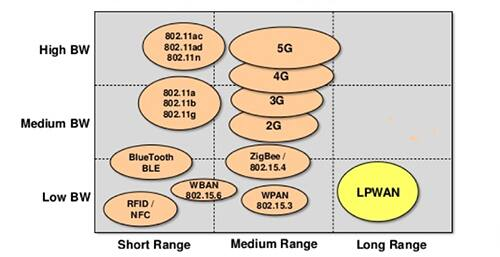
\includegraphics[width=0.9\textwidth]{img/lpwan.jpg}
    \label{fig:lpwan}
    
    Fonte: Link Labs, Peter R. Egli, 2015.
\end{figure}

\subsection{Tecnologias LPWAN existentes}

Atualmente existem diversas tecnologias LPWAN e elas podem ser divididas em duas categorias: espectro
aberto, e espectro licenciado. Isso significa que algumas tecnologias LPWAN operam numa faixa de frequência que é necessário pagar para o uso, e outras usam a faixa de frequência livre de diversos
países, porem isso implica em determinados países algumas regras de uso e também o compartilhamento
da faixa com outros dispositivos. Dentre as tecnologias mais famosas podem ser destacadas a NB-IoT,
Sigfox e LoRa, presentes em diversas soluções IoT de longas distâncias. Na figura \ref{fig:lpwans}
a seguir é possível visualizar algumas das tecnologias LPWAN. \cite{fi12030046}

\begin{figure}[H]
    \centering
	\caption{Tecnologias LWPAN}
    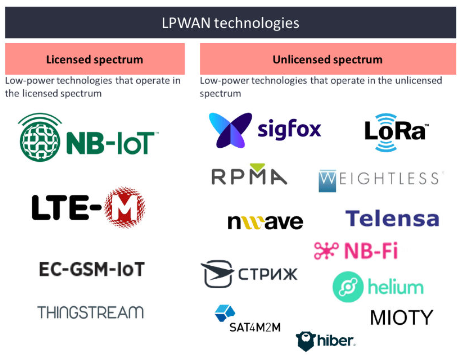
\includegraphics[width=0.7\textwidth]{img/lpwans.png}
    \label{fig:lpwans}
    
    Fonte: IoT Analytics LPWAN Mark Report 2018 - 2023, Romeo, 2019.
\end{figure}

\section{LoRa}

LoRa é uma tecnologia LPWAN que significa Long Range, foi criada em 2008 pela Cycleo SAS e adquerida
em 2012 pela Semtech, e é atualmente mantida pela LoRa Alliance. LoRa usa bandas de radiofrequência
sub-gigahertz de livre uso que podem variar entre 433 MHz, 868 MHz, 915 MHz e 923 MHz dependendo do
país. A tecnologia LoRa implementa uma camada física de comunicação, deixando aberto assim para outras
tecnologias cobrirem a responsabilidade das camadas acima, a mais conhecida para isso atualmente é a LoRaWAN, um protocolo de controle de acesso ao meio também mantido pela LoRa Alliance.  \cite{8474715}

\newpage

\subsection{Modulação LoRa}

A modulação LoRa é proprietária da Semtech e baseada em CSS, do inglês Chirp Spread Spectrum.
Diferente de modulações mais convencionas como FSK (Frequency-shift keying) que codifica
os símbolos para frequências especificas, a modulação LoRa codifica seus símbolos baseando-se no
incremento linear da frequência, gerando o que é chamado de "chirp". Na figura \ref{fig:lora1}
a seguir é possível ver esse "chirp" no domínio da franquênia e como é o sinal no domínio do
tempo. \cite{8067462}

\begin{figure}[H]
    \centering
	\caption{Chirp Spread Spectrum: Domínio da Franquênia e Domínio do Tempo}
    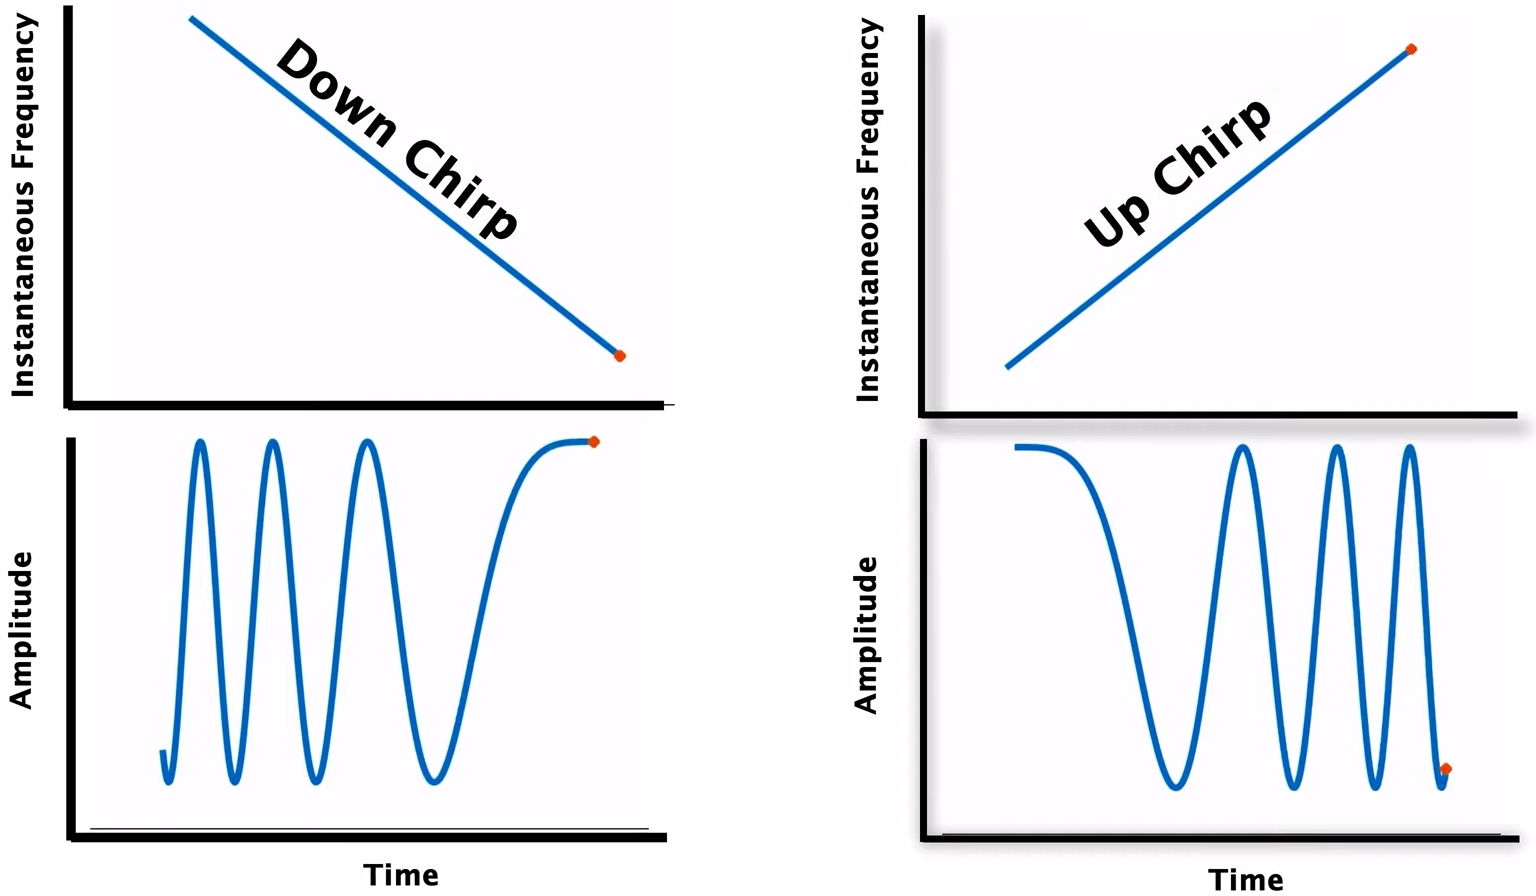
\includegraphics[width=0.7\textwidth]{img/lora1.png}
    \label{fig:lora1}
    
    Fonte: Visual Electric Youtube Channel, 2021.
\end{figure}

Na figura \ref{fig:lora2} a seguir, podemos ver uma representação matemática de uma sinal na modulação LoRa,
apesar de relativamente complexa, podemos analisa-lá de uma maneira mais simplória para entender como
a Tecnologia LoRa gera diferentes "chirps" para codificar os símbolos.

\begin{figure}[H]
    \centering
	\caption{Representação matemática de um sinal LoRa}
    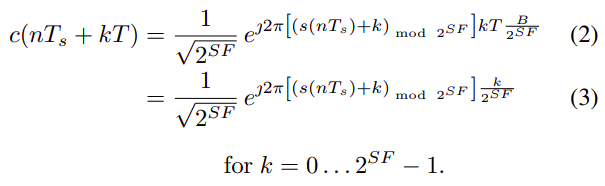
\includegraphics[width=0.8\textwidth]{img/lora2.png}
    \label{fig:lora2}
    
    Fonte: Frequency Shift Chirp Modulation: the LoRa™ Modulation, Lorenzo Vangelista, 2017.
\end{figure}

Focando apenas na exponencial complexa, sabemos pela matemática que isso representa uma onda senoidal,
onde a frequência base é determinada por \(s(nT_{s})\) e gradualmente incrementada por \(k\), e isso por
si só já forma o "chirp" visto na figura \ref{fig:lora1}. O grande truque está no \(\mod 2^{SF}\), esse
módulo garante que a frequência incremente até o limite superior da largura de banda, e volte para o limite
inferior, gerando assim uma descontinuidade no "chirp" que pode ser visto na figura \ref{fig:lora3-4} a
seguir. \cite{8067462}

\begin{figure}[H]
    \centering
        \caption{Modulação LoRa: Descontinuidade e Largura da Banda}
        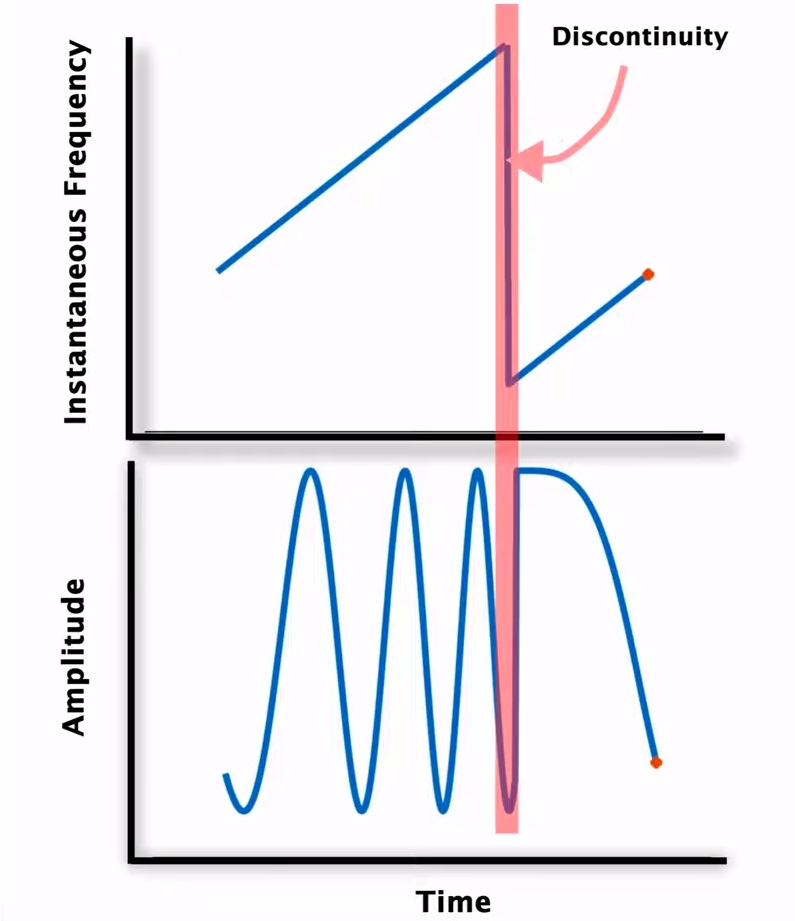
\includegraphics[width=.4\linewidth]{img/lora3.png}
        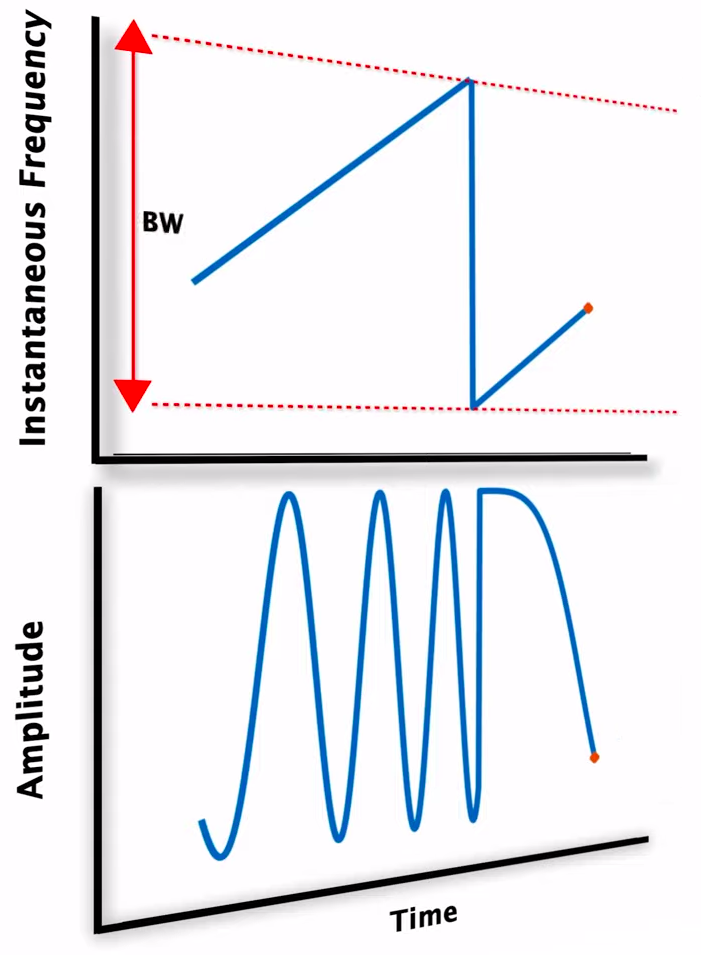
\includegraphics[width=.35\linewidth]{img/lora4.png}
    \label{fig:lora3-4}

    Fonte: Visual Electric Youtube Channel, 2021.
\end{figure}

Dessa forma, a codificação de um símbolo na modulação LoRa se encontra em qual momento dentro da
duração de um sinal ocorre essa descontinuidade. Na figura \ref{fig:lora5} seguir podemos ver
alguns exemplos de sinais LoRa com diferentes momentos de descontinuidade.

\begin{figure}[H]
    \centering
	\caption{Exemplos de Símbolos LoRa}
    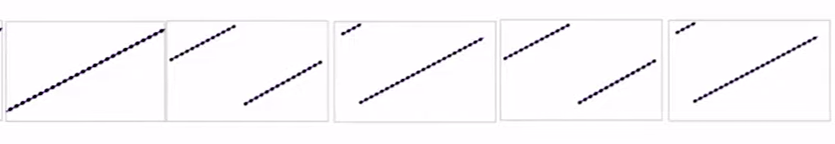
\includegraphics[width=0.8\textwidth]{img/lora5.png}
    \label{fig:lora5}
    
    Fonte: Visual Electric Youtube Channel, 2021.
\end{figure}

Esse tipo de modulação tem suas vantagens e desvantagens, a principal vantagem é robustez do sinal
a longas distâncias, e a principal desvantagem é que, por toda largura de banda ser usada para a codificação de cada símbolo, isso implica numa taxa da envio de dados mais baixa quando comparado
a outras modulações.

Uma característica importante na modulação LoRa é o termo SF visto na função do módulo, ele significa
"Spreading Factor" e representa um numero inteiro que pode ser de 7 a 12. o Spreading Factor determina
duas coisas importantes: a duração de um símbolo, e a quantidade possíveis de símbolos que podem ser
codificados. Quanto maior o Spreading Factor maior é o tempo para enviar um símbolo e maior também é
a quantidade símbolos. Na figura \ref{fig:lora6} a seguir podemos ver uma comparação entre os Spreading
Factors. \cite{8067462}

\newpage

\begin{figure}[H]
    \centering
	\caption{LoRa Spreading Factor}
    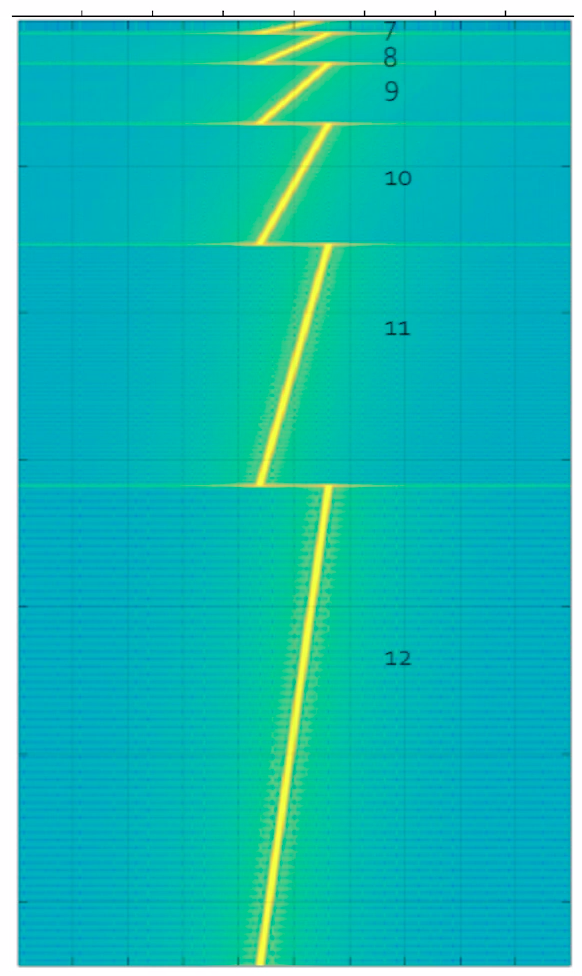
\includegraphics[width=0.32\textwidth]{img/lora6.png}
    \label{fig:lora6}
    
    Fonte: Richard Wenner Youtube Channel, 2017.
\end{figure}

Outra característica influenciada pelo Spreading Factor é a taxa de envio de dados, que diminui a
medida que o SF aumenta, pelo simples fato de que o envio de cada símbolo dura mais tempo, mas também
se aumenta a robustez do sinal.

Como o momento em que a descontinuidade ocorre no "chirp" é um ponto essencial para a decodificação,
o receptor precisa de certa forma saber identificar quando é o começo e o final de um sinal. Para isso
existe o que é chamado de "Preamble", que é um conjunto de sinais idênticos que são enviados uma quantidade fixa de vezes antes de qualquer dado significativo, funcionando assim como um tipo de sincronização. Na figura \ref{fig:lora7} a seguir é possível ver uma exemplo. \cite{8067462}

\begin{figure}[H]
    \centering
	\caption{LoRa Preamble}
    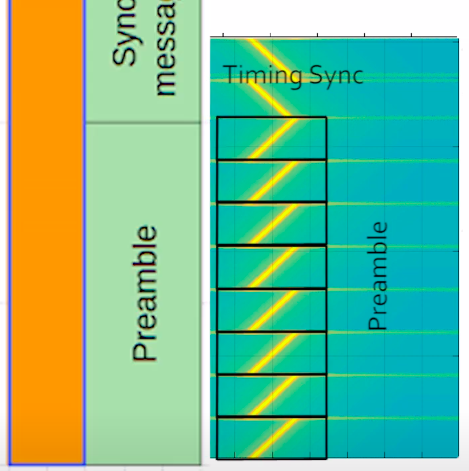
\includegraphics[width=0.34\textwidth]{img/lora7.png}
    \label{fig:lora7}
    
    Fonte: Richard Wenner Youtube Channel, 2017.
\end{figure}

\newpage

Na figura \ref{fig:lora8-9} a seguir é possível ver a estrutura de um Frame LoRa e um exemplo
de um frame no domínio da frequência.

\begin{figure}[H]
    \centering
	\caption{LoRa Frame}
    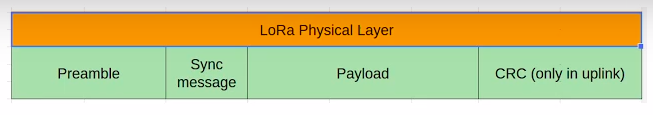
\includegraphics[width=0.8\textwidth]{img/lora8.png}

    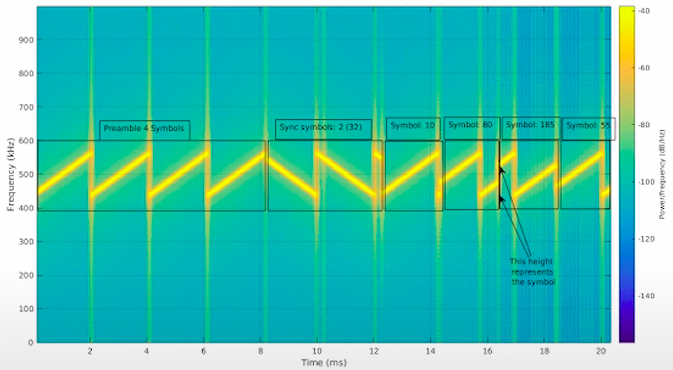
\includegraphics[width=0.8\textwidth]{img/lora9.png}
    \label{fig:lora8-9}
    
    Fonte: Richard Wenner Youtube Channel, 2017.
\end{figure}

\newpage

\section{Protocolos de Controle de Acesso ao Meio}

Protocolos de Controle de Acesso ao Meio, ou do inglês Medium Access Control (MAC), são
protocolos responsáveis por administrar o funcionamento dos hardwares que compõem a camada
física de transmissão de dados, protocolos MAC fazem parte da segunda camada, a camada de
enlace, do modelo OSI, que pode ser vista na figura \ref{fig:osi} a seguir. \cite{5340799}

\begin{figure}[H]
    \centering
	\caption{Camadas do modelo OSI}
    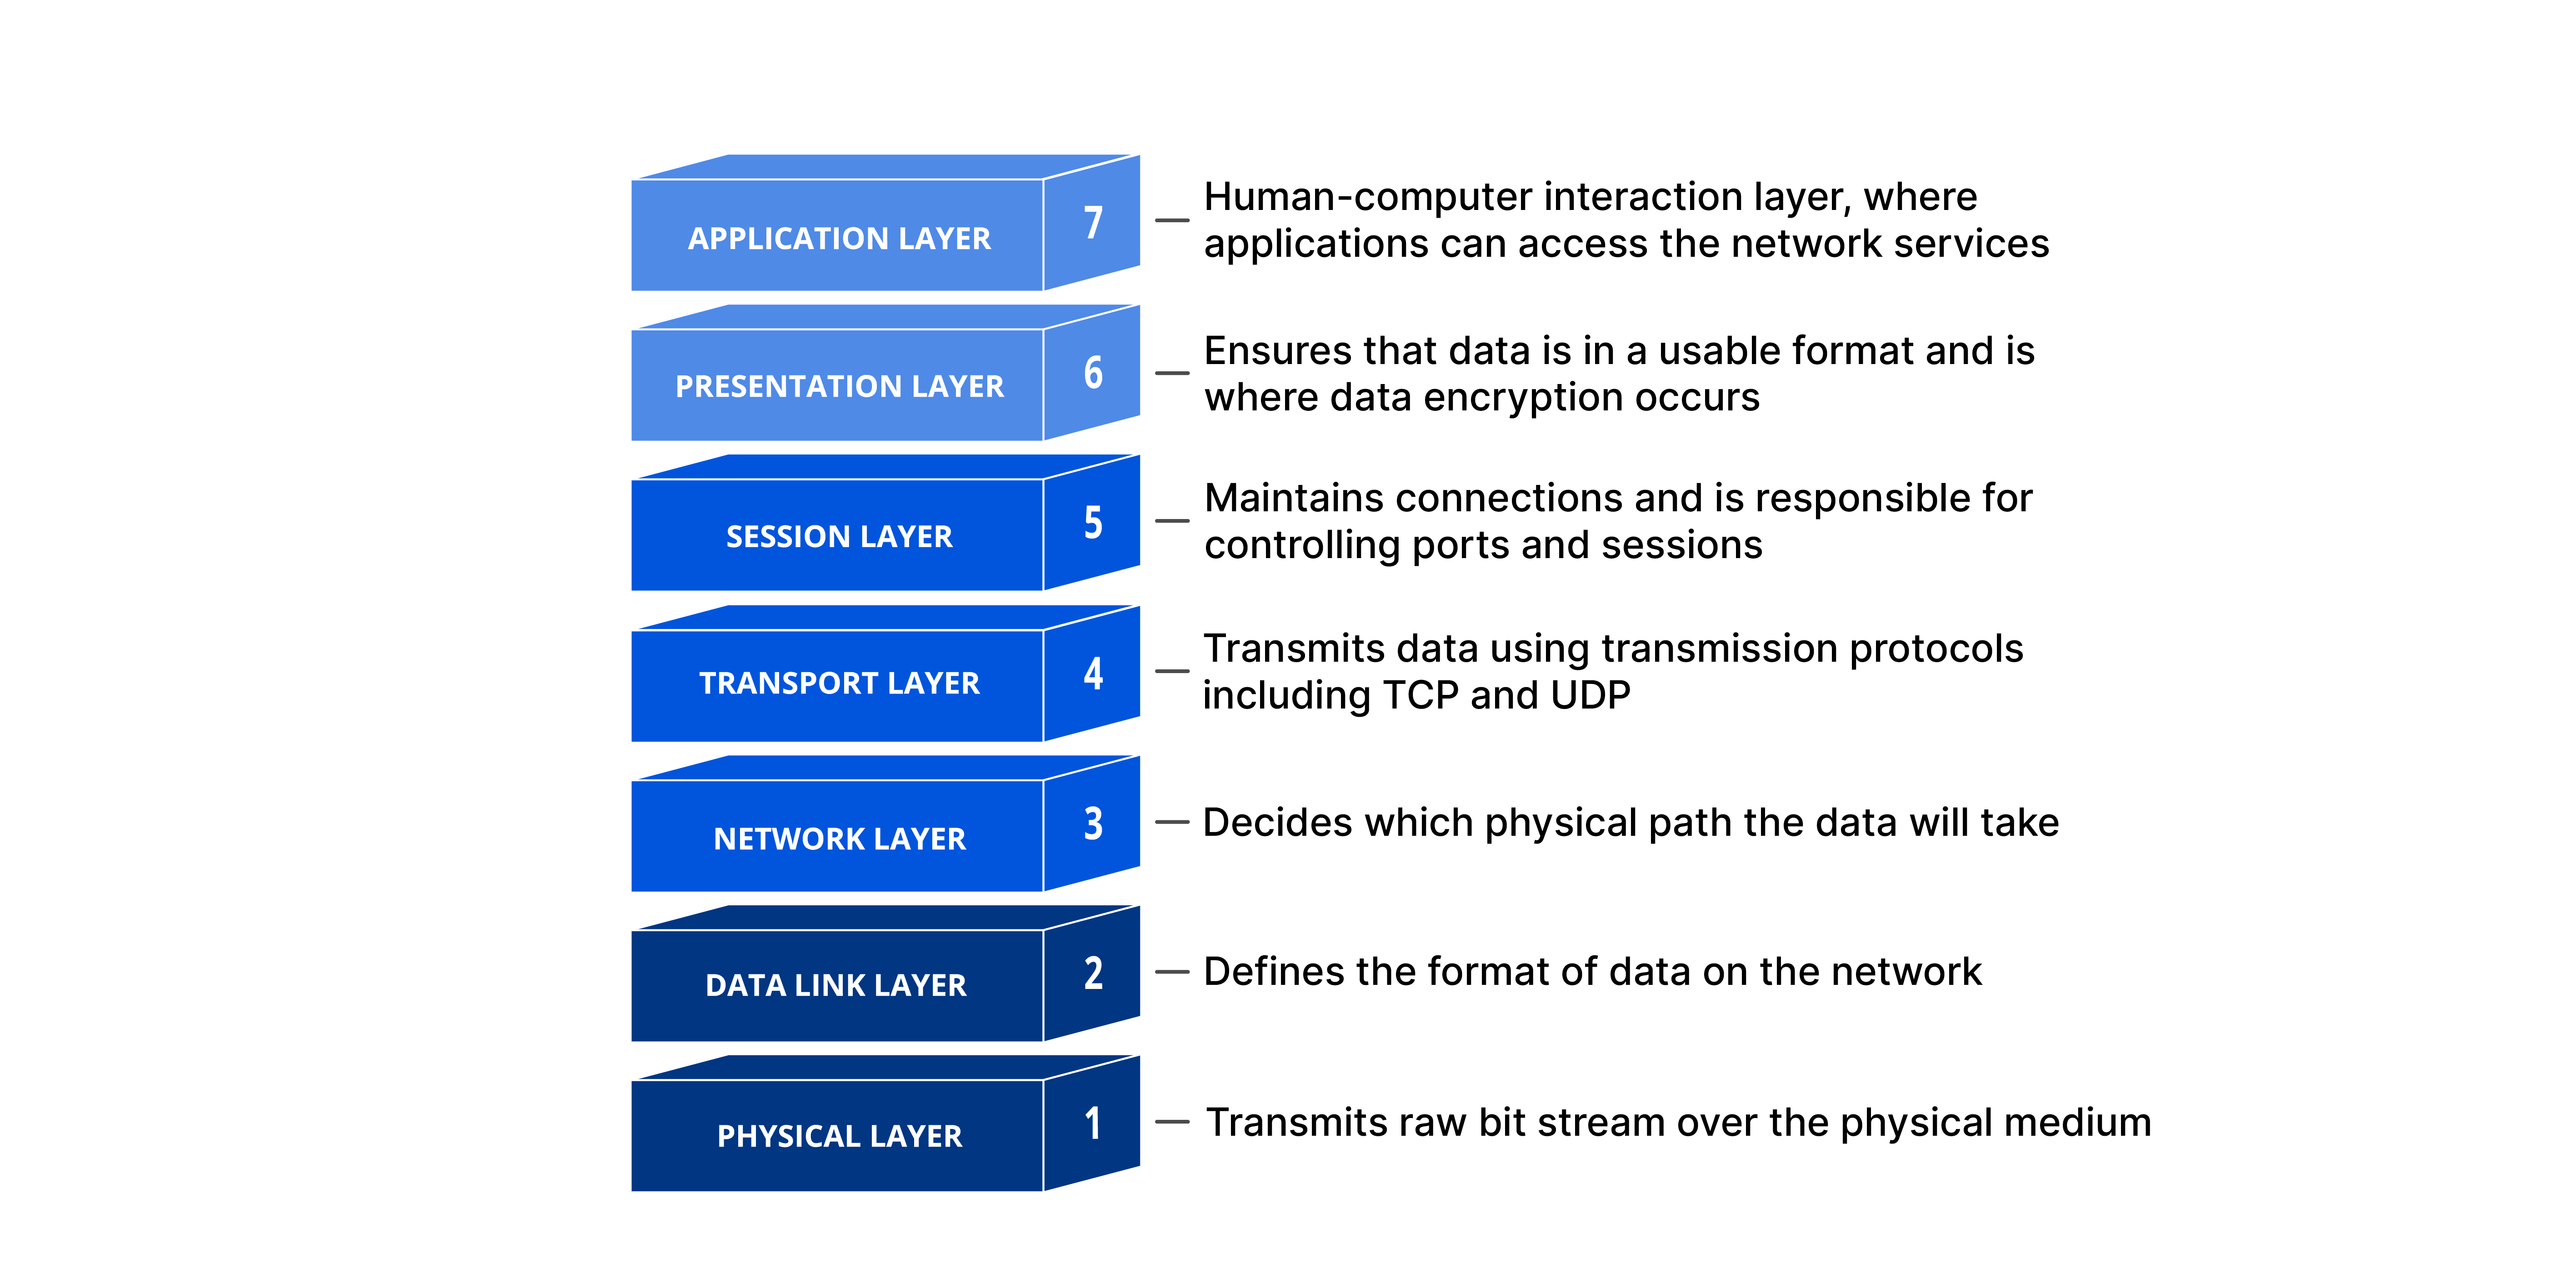
\includegraphics[width=0.9\textwidth]{img/osi-model.png}
    \label{fig:osi}
    
    Fonte: Cloudflare, 2022.
\end{figure}

\subsection{Características de Protocolos MAC}

Protocolos MAC em geral gerenciam o controle de fluxo e a multiplexação de um meio
de comunicação, provendo uma de qualidade de serviço para a camada inferior. Das
características dos protocolos MAC duas mais se destacam: \cite{5340799}

\begin{itemize}
    \item \textbf{Tratamento de Colisão:} Por o canal de comunicação ser normalmente
    compartilhado por outros dispositivos, é normal acontecer colisões, que ocorrem
    quando mais de um dispositivo tentam enviar dados ao mesmo tempo. Cabe ao protocolo
    MAC administrar a vez de uso de cada dispositivo no canal, e também administrar uma
    solução em casos onde pacotes colidem.
    \item \textbf{Detecção de Erros:} Pela natural física de alguns canais de comunicação,
    principalmente os sem fio, é possível que dados que saiam do remetente para o destinatário
    e cheguem corrompidos, assim cabe ao protocolo MAC ter mecanismos de detecção para
    quando esses erros acontecem.
\end{itemize}

\subsection{Exemplos de Algoritmos}

Existem alguns algoritmos conhecidos que garantem as características de um Protocolo MAC,
entre eles temos: \cite{5340799}

\begin{itemize}
    \item \textbf{ALOHA:} O algoritmo ALOHA é um dos mais antigos, surgir na década de 70
    e se destaca pela sua simplicidade: Se você tem dados para mandar, envie-os, Se ocorrer colisão, tente enviar novamente mais tarde. Outra característica desse algoritmo é a divisão
    do dados em pacotes menores que são enviados entre um determinado intervalo de tempo, com isso
    impedia que um único Nó ocupe o canal infinitamente.
    \item \textbf{CSMA/CD:} do inglês Carrier Sense Multiple Access with Collision Detection,
    é um algoritmo mais sofisticado com mecanismo de detecção de colisão. Quando um Nó durante
    a transmissão detecta uma colisão ele imediatamente para a transmissão e enviar um Frame
    de erro, para avisar a todos os nós do canal que houve uma colisão, impedindo que outros
    Nós tentem enviar algum dado. Os Nós que desejam enviar algum pacote deverão esperar um tempo
    aleatório cada para começarem uma nova transmissão.
    \item \textbf{CSMA/CA:} Já o CSMA/CA, do inglês Carrier Sense Multiple Access with Collision Avoidence, utiliza de sinal RTS (Request to Send) e CTS (Clear to Send). Qualquer Nó que
    deseja fazer uma transmissão manda um sinal RTS e só poderá começar o envio após receber
    um CTS, qualquer outro Nó ao perceber esses sinais no canal evitam fazer uma transmissão
    por um determinado período de tempo.
    \item \textbf{Token Ring:} O algoritmo Token Ring foi criado na década de 60 pela IBM e
    apenas funciona em redes com topologia Anel, é uma algoritmo simples onde um token é passado
    de Nó a Nó e apenas quem está com o Token pode transmitir. Se um Nó com o Token não deseja
    transmitir, ele transfere o Token para o próximo Nó, além disso cada Nó pode ficar com o
    Token por um determinado tempo.
\end{itemize}
\chapter{Trabalhos Relacionados}

Nesse capítulo será apresentado alguns trabalhos em torno do tópico de desenvolvimento
de protocolos para rádios LoRa. Será feita um breve descrição dos trabalhos existentes,
uma explicação dos critérios que serão considerados ao comparar os projetos, e por fim, a
análise comparativa em si.

\section{LoRaCTP}

Lora Content Transfer Protocol, ou como chamado pelos criadores de LoRaCTP, é um 
protocolo baseado em LoRa para a transferência do que eles chamam de "conteúdos" entre dispositivos LoRa de maneira confiável, no sentido em que todos os dados que saírem do
remetente chegarão no destinatário. O projeto foi publicado em 2020 por K. Nakamura, P. Manzoni, M. Zennaro, J. -C. Cano e C. T. Calafate, 4 membros da Universidade Politécnica de Valência na 
Espanha e 1 membro do Centro Internacional de Física Teórica na Itália. O trabalho teve
como objetivo implementar um protocolo em cima da camada LoRa para a transferência de "conteúdos", que são simplesmente qualquer dado arbitrário de diferentes tamanhos, entre dois dispositivos com um rádio LoRa. Para atingir esse objetivo o protocolo divide o
conteúdo a ser envido em N pacotes, cada um com um tamanho fixo e 
abaixo do limite máximo que a modulação LoRa suporta. Cada um desses pacotes é encapsulado com um cabeçalho de 20 bytes, com informações do endereço do remetente, endereço do destinatário, flags e checksum. Para garantir o objetivo principal que é a entrega
de todos os pacotes ao destinatário, o protocolo segue a metodologia "stop-and-wait"
onde é enviado um pacote, e o próximo da sequência só será enviado após uma confirmação de
recebimento do destinatário dentro de 5 segundos. Os pacotes dessa forma devem ser enviados na ordem correta e no caso de falha de algum envio é feita no máximo 3 tentativas de 
retransmissão até ser considerado que existe algum problema no canal como ruído ou simplesmente ocupado, e a tentativa de envio do conteúdo é dada como falha. Entretanto o 
trabalho não entra em detalhes sobre o fluxo completo da transmissão dos dados, como se 
existe algum handshake antes da transmissão, e que metadados são trocados nesse handshake. LoRaCTP em teoria aceita conteúdos de tamanho ilimitados, mas no trabalho foi testado
conteúdos de até 150 Kbytes a uma distância de até 6 Km. O hardware utilizado para os testes
foi um LoPy4, uma placa de desenvolvimento embarcado com MicroPython e suporte para 4 diferentes tectonologias de rádio, LoRa, SigFox, WiFi e Bluetooth. O protocolo foi desenvolvido na linguagem Python e aberto ao público no Github. \cite{9394317}

\newpage

\section{LoRaMesher}

\begin{figure}[H]
    \centering
	\caption{LoRaMesher: ESP32 com LoRa numa rede Mesh}
    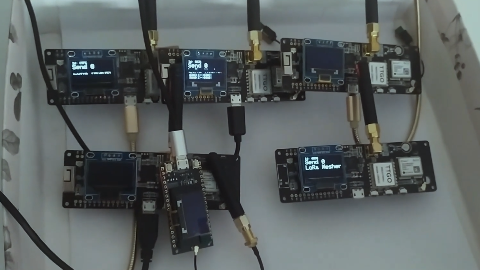
\includegraphics[width=0.6\textwidth]{img/loramesher.png}
    \label{fig:loramesher}
    
    Fonte: Implementation of a LoRa Mesh Library, 2022.
\end{figure}

Em outubro de 2022, Joan Miquel Solé, Roger Pueyo Centelles, Felix Freitag e Roc Meseguer publicaram
pela IEEE um trabalho chamado de "Implementation of a LoRa Mesh Library". A principal motivação dos
pesquisadores foi em notar que grande maioria das aplicações IoT com LoRa usam a arquitetura LoRaWAN
que possui limitações, como a de Nós finais da arquitetura não poderem se comunicar diretamente entre si mesmo quando a tecnologia LoRa fornece esse total suporte. Com isso, o objetivo principal dos
pesquisadores foi desenvolver uma arquitetura de rede alternativa ao LoRaWAN para dispositivos IoT
que melhor utilize os recursos da tecnologia LoRa. Os pesquisadores derem o nome para a implementação
de "LoRaMesher", uma biblioteca escrita em C++ desenvolvida para o microcontrolador ESP32 com chip LoRa
integrado. A biblioteca implementa uma topologia de rede Mesh e utiliza de APIs do FreeRTOS para
gerenciar recursos de memorias e processamento necessários para o protocolo. Foi implementado uma
metologia de transmissão confiável parecida com o "stop-and-wait" porém o protocolo é capaz de
calcular um tempo aproximado para que cada pacote de dado chegue no seu destinatário. Além disso foi
implementado um mecanismo de tratamento de colisão baseado no CSMA/CA, onde cada Nó primeiro verifica
se o canal está livre, para tentar utiliza-ló. A biblioteca tem código aberto e está disponível no Github para contribuição e uso, além disso ela possui uma pequena pagina Wiki para ajudar desenvolvedores que estão começando a utiliza-lá. No geral, o LoRaMesher é uma boa alternativa
para desenvolvedores IoT que precisam de mais flexibilidades de Rede no qual o LoRaWAN não suporta.
Pórem o LoraMesher pode apenas ser utilizado em microcontroladores IoT ESP32 com chip LoRa integrado,
além de que não tem implementado nenhum processo de empacotamento dos dados, implicando que se o
desenvolvedor necessita mandar mensagens maiores do que o payload do LoRaMesher suporta, ele
mesmo terá que implementar seu mecanismo de quebra de mensagens e empacotamento por cima do
LoRaMesher. \cite{9930341}

\newpage

\section{Critérios Comparativos}

Nesse capítulo foram escolhidos algumas características que serão levadas em consideração ao se comparar os trabalhos apresentados aqui. Nessa seção será apresentados esses critérios e suas descrições.

\begin{itemize}
    \item \textbf{Topologia de Rede:} A topologia de rede define de que forma os elementos de uma rede
    estão organizados, quais nós estão interligados e quais não estão, com isso surge diferentes possibilidades e também limitações para os fluxo de dados entre os participantes da rede. Segue algumas topologias existentes: Estrela, Mesh, Anel, Barramento, Estrela de Estrelas.
    \item \textbf{Transmissão Confiável:} Transmissão confiável é a existência de qualquer processo que
    garanta ou tente garantir que todos os dados enviados pelo destinatário chegaram no remetente. Um exemplo clássico são os protocolos da camada de transporte TCP e UDP, onde o TCP possui mecanismos de verificação se um pacote chegou no remetente, mas já o UDP simplesmente envia o pacote sem mecanismo algum de saber se ele foi recebido ou não.
    \item \textbf{Tratamento de Colisão:} Independente do canal de comunicação, sempre haverá uma limitação em relação ao dados que podem estar presentes no canal num determinado período de tempo, e a quebra
    desse limite implica na corrupção dos dados, da mesma forma em que dois humanos não conseguiriam se entender se os dois falassem ao mesmo tempo um com o outro. Assim, o tratamento de colisão é a existência de qualquer processo que trate ou evite colisões de dados dentre de um determinado canal
    de comunicação. Segue alguns protocolos conhecidos para isso: ALOHA, CSMA/CD, CSMA/CA, Token Ring.
    \item \textbf{Empacotamento:} Assim como o canal possui uma limitação de uso temporal, existe também
    uma limitação de banda, que significa o quão grande podem ser os dados para trafegarem nesse canal. Assim, empacotamento significa a existência de qualquer processo que divida uma mensagem inteira em N pacotes menores para que possa ser respeitado o limite de banda do canal.
    \item \textbf{Integridade dos Dados:} Integridade dos dados é a existência de qualquer processo que
    garanta que os dados enviados para o remetente chegaram exatamente idênticos aos enviados.
    \item \textbf{Independente do Rádio:} Independente do rádio significa se os trabalhos propostos
    foram implementados para funcionar em qualquer que seja o hardware e o rádio LoRa.
    \item \textbf{Biblioteca para Uso:} Biblioteca para uso significa se os autores do trabalho
    disponibilizaram as funcionalidades implementadas encapsuladas de alguma forma como uma biblioteca
    de programação para serem testadas e/ou usadas por terceiros.
    \item \textbf{Código Aberto:} Código Aberto significa se os autores do trabalho disponibilizaram
    o código fonte das suas implementações abertos para modificação e/ou contribuição de terceiros.
\end{itemize}

\section{Análise Comparativa}

\begin{table}[H]
    \begin{center}
    \caption{Comparativo entre trabalhos relacionados}
    \label{table:rel-comp}
    \begin{tabular}{|l|l|l|l|}
    \hline
     & LoRaCTP & LoRaMesher \\
    \hline
    Topologia de Rede & Nenhuma & Mesh \\
    \hline
    Transmissão Confiável & Sim & Sim \\
    \hline
    Tratamento de Colisão & ALOHA & CSMA/CA \\
    \hline
    Empacotamento & Sim & Não \\
    \hline
    Integridade dos Dados & Checksum de 3 bytes & Nenhum \\
    \hline
    Independente do Rádio & Não & Não \\
    \hline
    Biblioteca para uso & Não & Sim \\
    \hline
    Código Aberto & Sim & Sim \\
    \hline
    \end{tabular}
    \end{center}
\end{table}
\chapter{Metodologia}

Neste capítulo será apresentado a metodologia utilizada para o desenvolvimento
dos objetivos propostos para o projeto. Primeiramente será descrito as etapas
definidas para do desenvolvimento do protocolo, onde cada etapa depende dos
resultados gerados nas etapas anteriores. De modo geral, as etapas podem ser
dividades em 2 fases. A primeira fase de idealização e visão geral, tem o
objetivo de entender e definir o escopo do problema assim como gerar documentações
que vão definir em alto nível o que é, e como funciona o protocolo proposto.
Já na segunda fase, fase de implementação, o objetivo é traduzir toda a
documentação gerada na fase anterior para ser executada e testada num sistema
embarcado. \newline

O processo criativo e de desenvolvimento do sistema proposto seguiu metodologias
inspiradas na literatura de engenharia de software. Para especificar as etapas
segue a Figura \ref{fig:es}.

\begin{figure}[h]
	\begin{center}
	\caption{Etapas do Desenvolvimento do Projeto Proposto}
    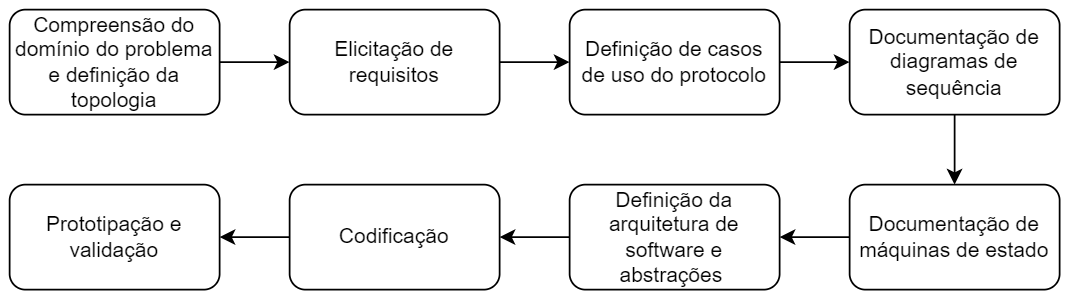
\includegraphics[width=\textwidth]{img/es.drawio.png}
    Fonte: Autor, 2022.
    \label{fig:es}
	\end{center}
\end{figure}

\section{Idealização e Visão Geral}

Vamos supor um cenário onde um desenvolvedor IoT está construindo um sistema
de monitoramento florestal. Ele deseja construir dispositivos embarcados que
monitorem diariamente certo aspecto da floresta e, ao sinal de qualquer mudança,
notifiquem um sistema Web. Porém essa floresta é extremamente remota, longe
de qualquer civilização e, dessa forma, \textbf{longe de fontes de energia e conectividade}.
Assim, ele precisa que seus dispositivos embarcados sejam \textbf{energicamente eficazes},
como também darem suporte para \textbf{enviar e receber mensagens do sistema a longas distâncias}.
O desenvolvedor pesquisa tecnologias no mercado e vê que LoRa pode ser uma solução para
esses problemas. Porém, apenas a adoção de rádios LoRa ao seu projeto não
fornece uma \textbf{infraestrutura de rede preestabelecida} para seus dispositivos, e agora ele se encontra
numa situação onde, além de desenvolver seu projeto principal, ele precisa
implementar alguma arquitetura de rede completa. Tomando esse exemplo como inspiração,
esse trabalho se propõe a
desenvolver um protocolo de rede baseado na tecnologia LoRa que forneça aos
desenvolvedores IoT uma implementação de rede compatível com suas necessidades
genéricas e que seja de fácil integração ao seu projeto atual.

Para definir a topologia da Rede deste projeto é preciso entender que, na maioria das vezes
pela questão remota, poucos dispositivos dessa rede tem a capacidade
de enviar ou receber algum dado pela Internet, logo esses dispositivos precisam
que \textbf{pelo menos 1} dispositivo da rede tenha essa capacidade para que os demais
enviem e recebam suas mensagens do sistema Web por meio deste. Esse dispositivo
recebe um nome especial de \textbf{"Gateway"}, e no geral sua função principal é de ser
essa ponte dos dispositivos locais com a Internet. Já os outros dispositivos recebem o nome de \textbf{"Nó"},
e no geral, é onde se encontra parte das funcionalidades do negócio do
desenvolvedor IoT. Dentre as topologias de Rede existentes, as topologias
\textbf{"Estrela"} e \textbf{"Mesh"} se destacam, cada uma com suas vantagens e desvantagens.
Para esse projeto foi escolhido a topologia Estrela, como pode ser vista
na Figura \ref{fig:topology}, principalmente pela sua simplicidade. Um 
comparativo mais detalhado pode ser visto na Tabela \ref{table:topology}.
\cite{9385408} \cite{9049146} \cite{8115793}

\begin{figure}[h!]
	\begin{center}
	\caption{Topologia de Rede Estrela}
    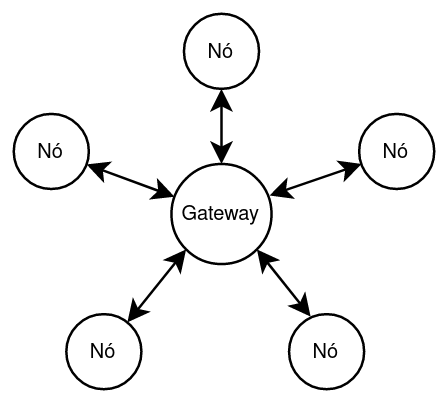
\includegraphics[width=0.31\textwidth]{img/topology.drawio.png}
    
    Fonte: Autor, 2022.
    \label{fig:topology}
	\end{center}
\end{figure}

\begin{table}[h!]
    \begin{center}
    \caption{Comparativo entre Topologia Estrela e Mesh}
    \label{table:topology}
    \begin{tabular}{|l|l|l|}
    \hline
     & Estrela & Mesh \\
    \hline
    Complexidade da Rede & Baixa & Alta \\
    \hline
    Consumo de energia nos Nós & Baixo & Moderado \\
    \hline
    Quantidade máxima de Nós & Máximo suportado pelo Gateway & Soma dos máximos suportados \\
    na Rede                  &                              & pelos dispositivos da Rede \\
    \hline
    Área de cobertura & Distância máxima comum & Soma das distâncias máximas \\
                    &  entre o Gateway e Nós & comuns entre os dispositivos \\
    \hline
    \end{tabular}
    \end{center}
\end{table}

\section{Elicitação de Requisitos}

Pela teoria de engenharia de software, a elicitação de requisitos é uma etapa
em que, ao compreender o escopo do problema, se procura criar uma documento
que descreva certas características que deverá ter na solução, como funcionalidades,
e restrições \cite{324822}. Esse documento contém uma lista de Requisitos
Funcionais e Não-Funcionais e será a primeira documentação formal do
projeto proposto nesse trabalho. Tais requisitos seguiram o padrão que pode
ser visto na Tabela \ref{table:req_model}.

\begin{table}[h]
    \begin{center}
    \caption{Representação de Requisitos Funcionais e Não-Funcionais}
    \label{table:req_model}
    \begin{tabular}{|c|l|}
    \hline
    \textbf{[Identificador Alfanumérico]} & \textbf{Descrição} \\
    \hline
    Nome do Requisito & Texto da Descrição \\
    \hline
    \end{tabular}
    \end{center}
\end{table}

\subsection{Requisitos Funcionais}

Os requisitos funcionais documentados na Tabela \ref{tab:rfs}, descrevem
as funcionalidades que o protocolo proposto nesse trabalho deve possuir. É importante
frisar que esse protocolo tem o objetivo de simplificar o trabalho do desenvolvedor IoT,
como descrito anteriormente, dessa forma o principal usuário do protocolo é a aplicação
do desenvolvedor.


\begin{longtable}{|p{3.5cm}|p{9.0cm}|}
    \caption{Requisitos Funcionais do Protocolo Proposto}\label{tab:rfs} \\
    
    \hline
    \textbf{[RF01]} & \textbf{Descrição} \\
    \hline
    Inicializar em modo de operação de \newline “Nó” & \
    Protocolo dá suporte a uma aplicação para definir seu modo de operação como um Nó na Rede \\
    
    \hline
    \textbf{[RF02]} & \textbf{Descrição} \\
    \hline
    Inicializar em modo de operação de \newline “Gateway” & \
    Protocolo dá suporte a uma aplicação para definir seu modo de operação como um Gateway na Rede \\
    
    \hline
    \textbf{[RF03]} & \textbf{Descrição} \\
    \hline
    Varredura de \newline Gateways ao alcance do Nó & \
    Protocolo dá suporte ao Nó de de fazer uma varredura na sua área de alcance por possíveis Gateways \\
    
    \hline
    \textbf{[RF04]} & \textbf{Descrição} \\
    \hline
    Estabelecer \newline conexão com o \newline Gateway & \
    Protocolo dá suporte ao Nó de estabelecer uma conexão contínua com um Gateway dentro de uma determinada área \\
    \hline
    \newpage
    \hline
    \textbf{[RF05]} & \textbf{Descrição} \\
    \hline
    Suportar \newline múltiplas conexões \newline simultâneas & \
    Protocolo dá suporte a múltiplos Nós conectados ao mesmo tempo num Gateway \\
    
    \hline
    \textbf{[RF06]} & \textbf{Descrição} \\
    \hline
    Suporte ao \newline envio de dados \newline dentro da Rede & \
    Protocolo dá suporte ao envio de dados entre os \newline elementos da rede \\
    
    \hline
    \textbf{[RF07]} & \textbf{Descrição} \\
    \hline
    Suporte ao recebimento de dados \newline dentro da Rede & \
    Protocolo dá suporte ao recebimento de dados entre os elementos da rede \\
    
    \hline
    \textbf{[RF08]} & \textbf{Descrição} \\
    \hline
    Garantia da \newline transmissão \newline dos dados & \
    Protocolo garante que todos os dados enviados irão chegar no destino desde que esteja estabelecida uma conexão durante a transmissão \\
    
    \hline
    \textbf{[RF09]} & \textbf{Descrição} \\
    \hline
    Comunicação entre \newline Nós por meio do \newline Gateway & \
    Protocolo dá suporte aos Nós conectados da Rede de trocarem mensagens entre si por meio do Gateway \\
    
    \hline
    \textbf{[RF10]} & \textbf{Descrição} \\
    \hline
    Verificação de \newline atividade do Nó & \
    Protocolo dá suporte ao Gateway de confirmar o status de “online” do seus clientes \\
    \hline
\end{longtable}

\subsection{Requisitos Não-Funcionais}

Os requisitos não funcionais documentados na Tabela \ref{tab:rnfs}, descrevem
as restrições das funcionalidades do protocolo proposto. Algumas delas impostas
para a simplificação do protocolo, mas uma delas, como a \textbf{[RNF02]}, por
uma limitação física da própria modulação LoRa implementada nos rádios.
\newline
\newline

\begin{longtable}{|p{3.5cm}|p{9.0cm}|}
    \caption{Requisitos Não-Funcionais do Protocolo Proposto}\label{tab:rnfs}\\
    \hline
    \textbf{[RNF01]} & \textbf{Descrição} \\
    \hline
    Dados de \newline tamanho máximo \newline de até 512 bytes & \
    Protocolo exige que o tamanho máximo dos dados trocadas entre elementos da Rede seja de até 512 bytes \\
    \hline
    \textbf{[RNF02]} & \textbf{Descrição} \\
    \hline
    Divisão dos dados em pacotes de até 256 bytes & \
    Protocolo exige que os dados sejam divididos em pacotes de até no máximo de 256 bytes devido a limitação estabelecida pela modulação LoRa \\
    \hline
    \textbf{[RNF03]} & \textbf{Descrição} \\
    \hline
    Máximo de \newline 255 elementos \newline por Rede & \
    Protocolo exige que a quantidade total de elementos numa Rede seja de 255 elementos, onde no máximo 1 Gateway e 254 Nós \\
    \hline
\end{longtable}

\section{Documentação dos Casos de Uso}

Os casos de uso definem as interações, e os objetivos de cada interação, entre atores e sistemas.
Os atores são os principais usuários de um sistema, podem ser desde pessoas até mesmo
programas. De modo geral, um documento de Casos de Uso define quem são os atores do sistema,
de que forma o sistema processa uma interação com os atores, e qual o objetivo das interações
\cite{malan2001functional}. Neste trabalho, o sistema será o protocolo baseado em LoRa,
e o único ator será a aplicação do desenvolvedor IoT, ela que irá usar das funcionalidades
do protocolo para atingir seus objetivos. A figura \ref{fig:use-cases} na página a seguir
apresenta o Diagrama geral de Casos de Uso proposto nesse trabalho. Está seção tem o objetivo
de documentar os Casos de Uso da proposta de acordo com a tabela
\ref{tab:use-cases-def} a seguir.

\begin{longtable}{|p{2.65cm}|l|}
    \caption{Representação dos Casos de Uso}\label{tab:use-cases-def}\\
    \hline
    \textbf{[Identificador]} & Nome do Caso de Uso \\
    \hline
    \textbf{Descrição} & Descrição sobre o caso de uso \\
    \hline
    \textbf{Atores} & Atores envolvidos na interação \\
    \hline
    \textbf{Pré-condições} & Estado do sistema antes da interação \\
    \hline
    \textbf{Pós-condições} & Estado do sistema após a interação \\
    \hline
    \textbf{Fluxo Normal} & Processamento principal da interação \\
    \hline
    \textbf{Fluxos Alt.} & Processamentos alternativos da interação \\
    \hline
    \textbf{RF Rel.} & Requisito implementado pelo caso de uso \\
    \hline
\end{longtable}

\newpage

\begin{figure}[htp]
    \centering
	\caption{Diagrama de Casos de Uso da proposta}
    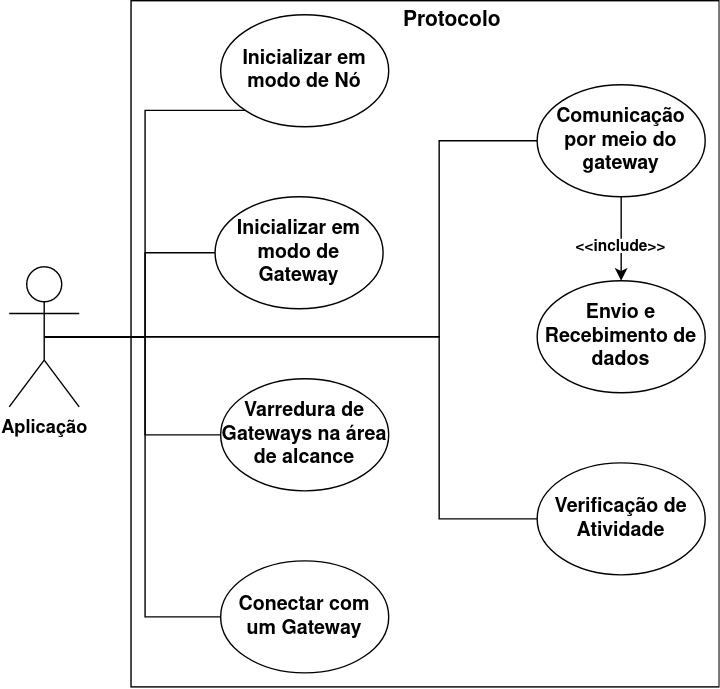
\includegraphics[width=0.6\textwidth,height=0.6\textheight,keepaspectratio]{img/use-cases.drawio.png}
    
    Fonte: Autor, 2022.
    \label{fig:use-cases}
\end{figure}

\begin{longtable}{|p{2.65cm}|p{13cm}|}
    \caption{Caso de Uso UC01}\label{tab:use-cases01} \\
    \hline
    \textbf{[UC01]} & Inicializar em modo de operação de Nó \\
    \hline
    \textbf{Descrição} & Aplicação solicita utilizar as funcionalidades do protocolo em modo de Nó. \\
    \hline
    \textbf{Atores} & Aplicação \\
    \hline
    \textbf{Pré-condições} & Nenhuma. \\
    \hline
    \textbf{Pós-condições} & 1. Protocolo informa que a inicialização foi bem sucedida. \\
    \hline
    \textbf{Fluxo Normal} & 1. Aplicação solicita ao protocolo a inicialização em modo de Nó, fornece seu 
    identificador único (UID) e a interface do rádio LoRa utilizado. \newline
    2. Protocolo informa que a inicialização em modo de Nó foi bem sucedida. \\
    \hline
    \textbf{Fluxos Alt.} & \
    Nenhum. \\
    \hline
    \textbf{RF Rel.} & \
    \textbf{RF01} \\
    \hline
\end{longtable}

\begin{longtable}{|p{2.65cm}|p{13cm}|}
    \caption{Caso de Uso UC02}\label{tab:use-cases02} \\
    \hline
    \textbf{[UC02]} & Inicializar em modo de operação de Gateway \\
    \hline
    \textbf{Descrição} & Aplicação solicita utilizar as funcionalidades do protocolo em modo de Gateway. \\
    \hline
    \textbf{Atores} & Aplicação \\
    \hline
    \textbf{Pré-condições} & Nenhuma. \\
    \hline
    \textbf{Pós-condições} & 1. Protocolo informa que a inicialização foi bem sucedida. \\
    \hline
    \textbf{Fluxo Normal} & 1. Aplicação solicita ao protocolo a inicialização em modo de Gateway, fornece seu identificador único (UID) e a interface do rádio LoRa utilizado. \newline
    2. Protocolo informa que a inicialização em modo de Gateway foi bem sucedida. \\
    \hline
    \textbf{Fluxos Alt.} & Nenhum. \\
    \hline
    \textbf{RF Rel.} & \textbf{RF02} \\
    \hline
\end{longtable}

\begin{longtable}{|p{2.65cm}|p{13cm}|}
    \caption{Caso de Uso UC03}\label{tab:use-cases03} \\
    \hline
    \textbf{[UC03]} & Varredura de Gateways na área de alcance \\
    \hline
    \textbf{Descrição} & Aplicação solicita ao Protocolo para fazer uma varredura de gateways na sua área de alcance. \\
    \hline
    \textbf{Atores} & Aplicação \\
    \hline
    \textbf{Pré-condições} & Protocolo deve ter sido inicializado em modo de Nó. \\
    \hline
    \textbf{Pós-condições} & 1. Protocolo fornece uma lista de Gateway ao seu alcance. \newline
    2. Protocolo informa que não há nenhum Gateway ao seu alcance. \\
    \hline
    \textbf{Fluxo Normal} & 1. Aplicação solicita ao Protocolo para fazer uma varredura por Gateways. \newline
    2. Protocolo no Nó envia um broadcast de um sinal solicitando a identificação dos gateways dentro do seu alcance e aguarda a resposta durante um determinado tempo. \newline
    3. Protocolo no Gateway recebe o broadcast e responde informando sua identificação. \newline
    4. Protocolo no Nó recebe como resposta do seu broadcast a identificação de cada Gateway ao seu alcance. \newline
    5. Protocolo no Nó fornece para a aplicação a lista de identificações dos Gateways ao seu alcance.\\
    \hline
    \textbf{Fluxos Alt.} & 3a. Se o Protocolo no Nó não recebe nenhuma resposta dentro do tempo esperado: \newline
    4a. Nó repete o passo 2 mais uma vez. \newline
    5a. Se novamente não for recebido nenhuma resposta: \newline
    6a. Protocolo no Nó informa que não há nenhum Gateway ao seu alcance. \\
    \hline
    \textbf{RF Rel.} & \textbf{RF03} \\
    \hline
\end{longtable}

\begin{longtable}{|p{2.65cm}|p{13cm}|}
    \caption{Caso de Uso UC04}\label{tab:use-cases04} \\
    \hline
    \textbf{[UC04]} & Conectar com um Gateway \\
    \hline
    \textbf{Descrição} & Aplicação Cliente solicita ao Protocolo para estabelecer conexão com um Gateway, e Aplicação Gateway recebe a nova conexão. \\
    \hline
    \textbf{Atores} & Aplicação Cliente e Aplicação Gateway \\
    \hline
    \textbf{Pré-condições} & Protocolo no Cliente deve ter sido inicializado em modo de Nó. \newline
    Protocolo no Gateway deve ter sido inicializado em modo de Gateway. \\
    \hline
    \textbf{Pós-condições} & 1. Protocolo no Cliente informa que a conexão foi estabelecida, e Protocolo no Gateway informa sobre a nova conexão. \newline
    2. Protocolo no Cliente informa que a conexão não foi estabelecida. \newline
    3. Protocolo no Cliente informa que o Gateway se encontra cheio. \\
    \hline
    \textbf{Fluxo Normal} & 1. Aplicação Cliente solicita ao Protocolo para conectar no Gateway com um identificação determinada. \newline
    2. Protocolo no Cliente envia um sinal de solicitação de conexão para o Gateway e fica no aguardo de uma resposta durante um determinado tempo. \newline
    3. Protocolo no Gateway recebe o sinal e verifica se pode aceitar a conexão. \newline
    4. Protocolo no Gateway responde ao sinal aceitando a conexão, envia o novo identificador de rede do Cliente e fica no aguardo de uma confirmação durante um determinado tempo. \newline
    5. Protocolo no Cliente recebe o sinal, atualiza o seu novo identificador da Rede, e confirma a atualização para o Gateway. \newline
    6. Protocolo no Cliente informa a Aplicação que a conexão foi estabelecida. \newline
    7. Protocolo no Gateway informa ao Gateway sobre a nova conexão. \\
    \hline
    \textbf{Fluxos Alt.} & 2a. Se o Protocolo no Cliente não recebe nenhuma resposta dentro do tempo esperado: \newline
    3a. Nó repete o passo 2 mais uma vez. \newline
    4a. Se novamente não for recebido nenhuma resposta, protocolo no Cliente informa a Aplicação
    que a conexão não foi estabelecida.
    \newline \newline \ 
    4b. Se o Protocolo no Gateway informar ao Cliente que está cheio: \newline
    5b. Protocolo no Cliente informa a Aplicação que o Gateway se encontra cheio no momento. \\
    \hline
    \textbf{RF Rel.} & \textbf{RF04} e \textbf{RF05} \\
    \hline
\end{longtable}

\begin{longtable}{|p{2.65cm}|p{13cm}|}
    \caption{Caso de Uso UC05}\label{tab:use-cases05} \\
    \hline
    \textbf{[UC05]} & Envio e Recebimento de dados \\
    \hline
    \textbf{Descrição} & Aplicação do Remetente solicita ao Protocolo para fazer envio de um dado para um Destinatário na Rede e Aplicação no Destinatário coleta o dado. \\
    \hline
    \textbf{Atores} & Aplicação do Remetente e Aplicação Destinatário \\
    \hline
    \textbf{Pré-condições} & Protocolo deve ter sido inicializado em ambos o Remetente e Destinatário. \newline
    Remetente e Destinatário devem estar conectados ao mesmo Gateway. \\
    \hline
    \textbf{Pós-condições} & 1. Protocolo no Remetente informa para a Aplicação que a transmissão foi bem sucedida e Aplicação Destinatário coleta o novo dado. \newline
    2. Protocolo no Remetente informa que a transmissão não foi bem sucedida. \\
    \hline
    \textbf{Fluxo Normal} & 1. Aplicação Remetente fornece para o Protocolo o dado a ser enviado e o identificador do Destinatário. \newline
    2. Protocolo no Remetente separa o dado em pacotes de tamanho máximo determinado, se necessário. \newline
    3. Protocolo no Remetente envia um pacote para o Protocolo no Destinatário solicitando o envio de dados e informando quantos pacotes serão enviados e aguarda um determinado tempo. \newline
    4. Protocolo no Destinatário recebe a solicitação e verifica se tem recursos sobrando para receber a transmissão. \newline
    5. Protocolo no Destinatário aceita a transmissão e envia um sinal para o Protocolo no Remetente para começar o envio dos pacotes e aguarda um tempo determinado.\newline
    6. Protocolo no Remetente envia pacote e aguarda confirmação de recebimento do Destinatário por um determinado tempo. \newline
    7. Protocolo no Destinatário recebe o pacote e envia confirmação de recebimento ao Remetente e aguarda o próximo pacote por um determinado tempo. \newline
    8. Repete-se o passo 6 ao 7 até que o ultimo pacote seja enviado. \newline
    9. Protocolo no Destinatário, após receber e confirmar o ultimo pacote, reconstrói os dados e informa a Aplicação Destinatário a chegada de novos dados. \newline
    10. Protocolo no Remetente recebe a confirmação do ultimo pacote recebido pelo destinatário e informa a Aplicação Remetente que o envio foi bem sucedido. \\
    \hline
    \textbf{Fluxos Alt.} & 3a. Se o Protocolo no Remetente não recebe uma resposta dentro do tempo determinado: \newline
    4a. Protocolo Remetente repete o passo 3 mais uma vez. \newline
    5a. Se novamente não for recebido nenhuma resposta, Protocolo no Remetente informa a Aplicação Remetente que o envio de dados não foi possível.
    \newline\newline
    4b. Se o Protocolo no Destinatário não tem recursos sobrando para receber a transmissão: \newline
    5b. Protocolo no Destinatário envia um sinal de recursos lotados. \newline
    6b. Protocolo no Remetente recebe a resposta de recursos lotados e informa a Aplicação Remetente que o Destinatário se encontra com recursos ocupados.
    \newline\newline
    6c. Se o Protocolo no Remetente não recebe o sinal de confirmação de recebimento pelo Destinatário: \newline
    7c. Protocolo no Remetente repete o envio do pacote mais uma vez e aguarda um tempo determinado. \newline
    8c. Se novamente não for recebido nenhum resposta, Protocolo no Remetente informa a Aplicação Remetente que o envio de dados não foi possível.
    \newline\newline
    7d. Se o Protocolo no Destinatário não recebe o próximo pacote dentro do tempo esperado: \newline
    8d. Protocolo no Destinatário envia sinal solicitando o reenvio do pacote esperado. \newline
    9d. Se novamente não for recebido nenhum pacote, Protocolo no Destinatário libera recursos alocados para a transmissão. \\
    \hline
    \textbf{RF Rel.} & \textbf{RF06}, \textbf{RF07}, \textbf{RF08} e \textbf{RF09} \\
    \hline
\end{longtable}

\begin{longtable}{|p{2.65cm}|p{13cm}|}
    \caption{Caso de Uso UC06}\label{tab:use-cases06} \\
    \hline
    \textbf{[UC06]} & Verificação de Atividade \\
    \hline
    \textbf{Descrição} & Aplicação Gateway solicita ao protocolo uma verificação de atividade de um determinado Nó. \\
    \hline
    \textbf{Atores} & Aplicação Gateway \\
    \hline
    \textbf{Pré-condições} & Protocolo no Gateway deve ter sido inicializado em modo de Gateway. \newline
    Aplicação Gateway deve ter estabelecido uma conexão com o Nó. \\
    \hline
    \textbf{Pós-condições} & 1. Protocolo no Gateway informa que o Nó está ativo. \newline
    2. Protocolo no Gateway informa que o Nó não está ativo. \\
    \hline
    \textbf{Fluxo Normal} & 1. Aplicação Gateway solicita ao protocolo uma verificação de atividade do Nó com um determinado identificador. \newline
    2. Protocolo no Gateway envia um sinal de verificação para o Nó e fica no aguardo de uma resposta por um determinado tempo. \newline
    3. Protocolo no Nó recebe o sinal e responde confirmando a atividade. \newline
    4. Protocolo no Gateway recebe a confirmação de atividade. \newline
    5. Protocolo no Gateway informa que o Nó está ativo. \\
    \hline
    \textbf{Fluxos Alt.} & 4a. Se o Protocolo no Gateway não recebe a confirmação de atividade: \newline
    5a. Protocolo no Gateway repete o passo 2 mais uma vez \newline
    6a. Se novamente não for recebido nenhuma resposta: \newline
    7a. Protocolo no Gateway informa que o Nó não está ativo. \\
    \hline
    \textbf{RF Rel.} & \textbf{RF10} \\
    \hline
\end{longtable}

\section{Documentação dos Diagramas de Sequência}

O diagrama de sequência é uma ferramenta visual que auxilia o melhor entendimento
das interações definidas na etapa de documentação dos casos de uso. Num diagrama
de sequencia é possível visualizar os fluxos dos casos com mais detalhe numa linha
temporal vertical e os diferentes módulos e atores que estão participando de determinado
fluxo. \newline

Está seção tem objetivo de documentar os diagramas de sequência dos casos de uso estabelecidos
na etapa anterior. A medida em que vamos melhor definindo as interações, mais nos aproximamos
de uma implementação real. Os diagramas a seguir, da Figura \ref{fig:sq-scan} até
\ref{fig:sq-alive-fa}, usam de funções e tipos de mensagens, essas funções e mensagens não
necessariamente representam a sua forma final quando implementada, mas sim tem o intuito
de ajudar o leitor do documento no entendimento do fluxo do diagrama.

\begin{figure}[htp]
    \centering
	\caption{Varredura de Gateways na área de alcance: Fluxo Normal}
    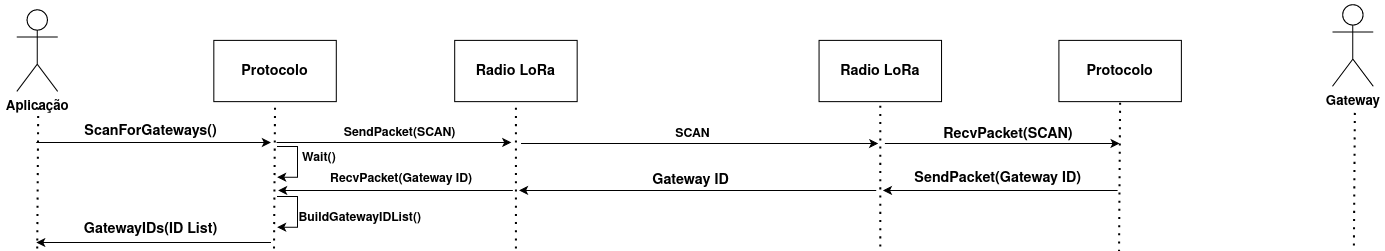
\includegraphics[width=\textwidth,height=0.14\textheight]{img/scan.drawio.png}
    \label{fig:sq-scan}
    Fonte: Autor, 2022.
\end{figure}

Diagrama baseado no caso de uso da tabela \ref{tab:use-cases03}.
\newpage

\begin{figure}[htp]
    \centering
	\caption{Varredura de Gateways na área de alcance: Fluxo Alternativo}
    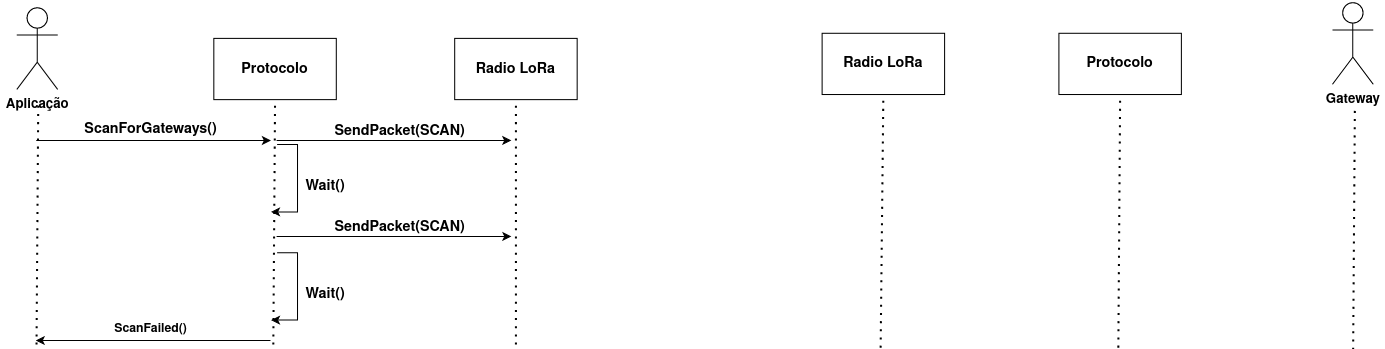
\includegraphics[width=\textwidth,height=0.17\textheight]{img/scan-fa.drawio.png}
    \label{fig:sq-scan-fa}
    Fonte: Autor, 2022.
\end{figure}

Diagrama baseado no caso de uso da tabela \ref{tab:use-cases03}.

\begin{figure}[htp]
    \centering
	\caption{Conectar com um Gateway: Fluxo Normal}
    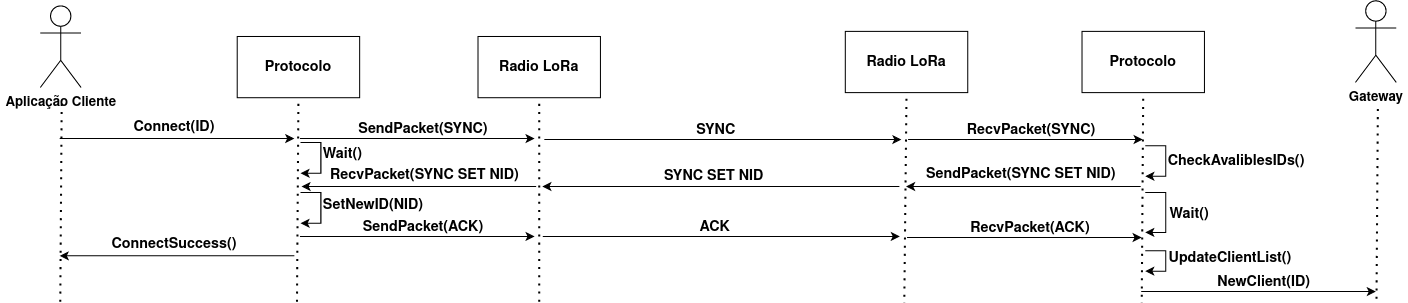
\includegraphics[width=\textwidth,height=0.18\textheight]{img/connect.drawio.png}
    \label{fig:sq-connect}
    Fonte: Autor, 2022.
\end{figure}

Diagrama baseado no caso de uso da tabela \ref{tab:use-cases04}.

\begin{figure}[htp]
    \centering
	\caption{Conectar com um Gateway: Fluxo Alternativo 1}
    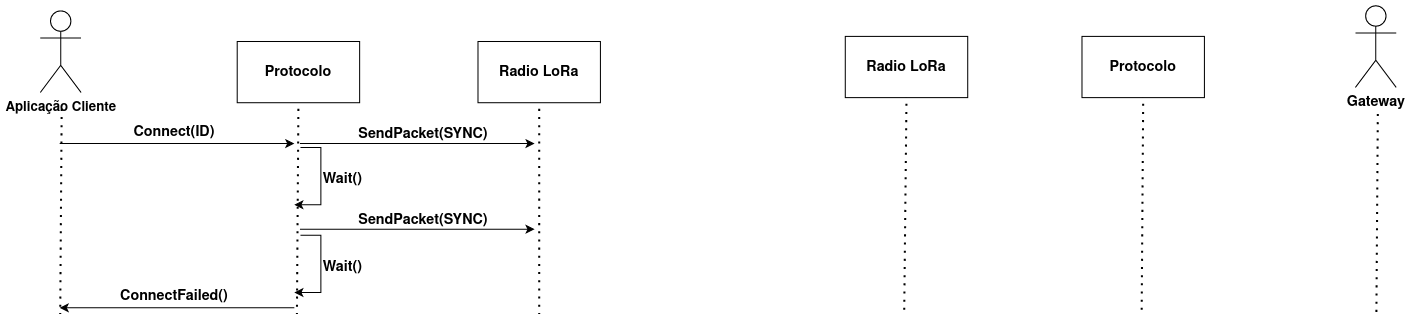
\includegraphics[width=\textwidth,height=0.14\textheight]{img/connect-fa2.drawio.png}
    \label{fig:sq-connect-fa}
    Fonte: Autor, 2022.
\end{figure}

Diagrama baseado no caso de uso da tabela \ref{tab:use-cases04}.
\newpage

\begin{figure}[htp]
    \centering
	\caption{Conectar com um Gateway: Fluxo Alternativo 2}
    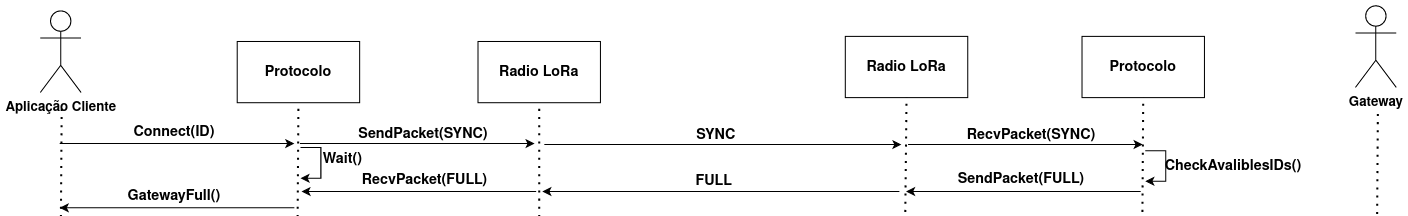
\includegraphics[width=\textwidth,height=0.09\textheight]{img/connect-fa.drawio.png}
    \label{fig:sq-connect-fa2}
    
    Fonte: Autor, 2022.
\end{figure}

Diagrama baseado no caso de uso da tabela \ref{tab:use-cases04}.

\begin{figure}[htp]
    \centering
	\caption{Envio e Recebimento de Dados: Fluxo Normal}
    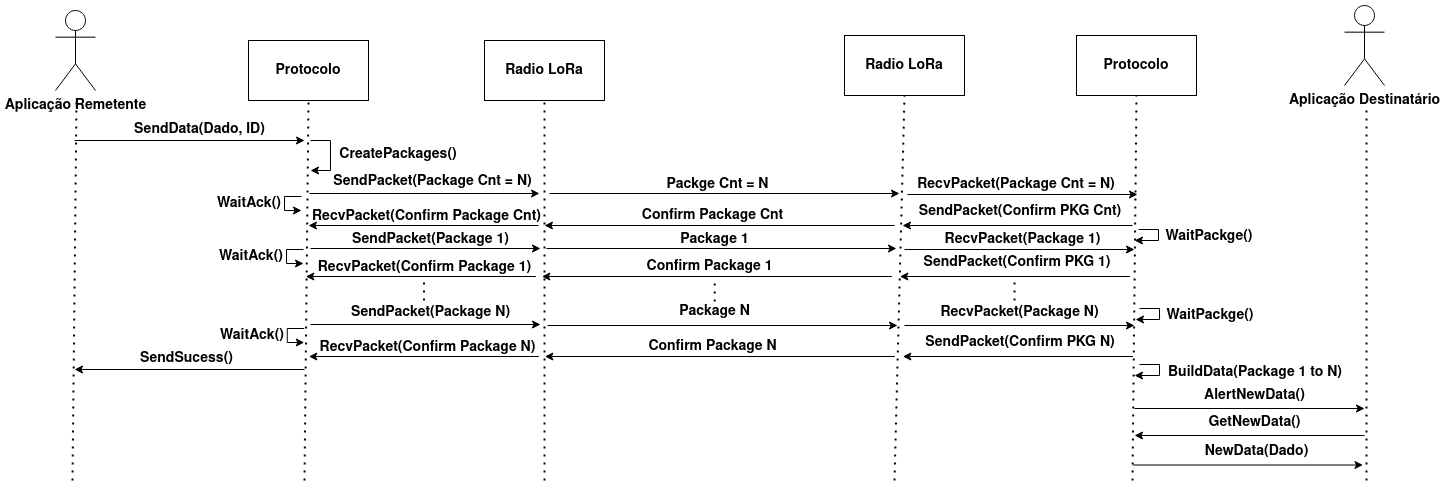
\includegraphics[width=\textwidth,height=0.27\textheight]{img/data.drawio.png}
    \label{fig:sq-data}
    Fonte: Autor, 2022.
\end{figure}

Diagrama baseado no caso de uso da tabela \ref{tab:use-cases05}.

\begin{figure}[htp]
    \centering
	\caption{Envio e Recebimento de Dados: Fluxo Alternativo 1}
    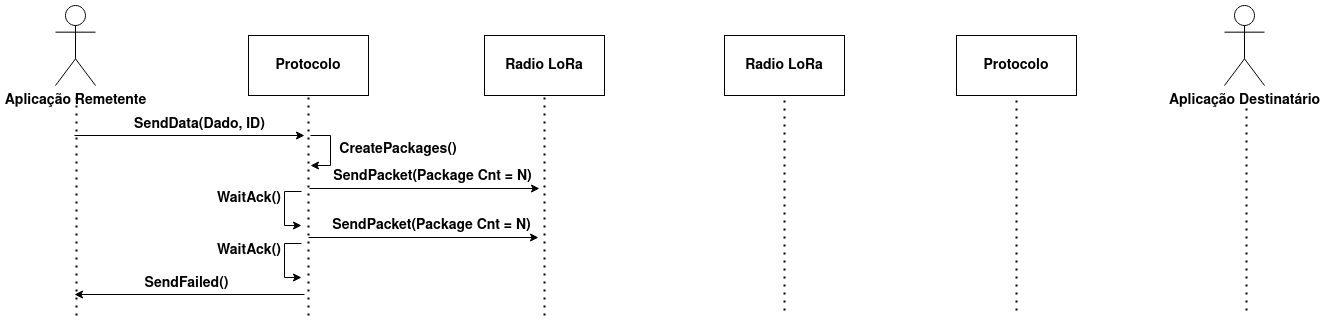
\includegraphics[width=\textwidth,height=0.13\textheight]{img/data-fa.drawio.png}
    \label{fig:sq-data-fa}
    Fonte: Autor, 2022.
\end{figure}

Diagrama baseado no caso de uso da tabela \ref{tab:use-cases05}.
\newpage

\begin{figure}[htp]
    \centering
	\caption{Envio e Recebimento de Dados: Fluxo Alternativo 2}
    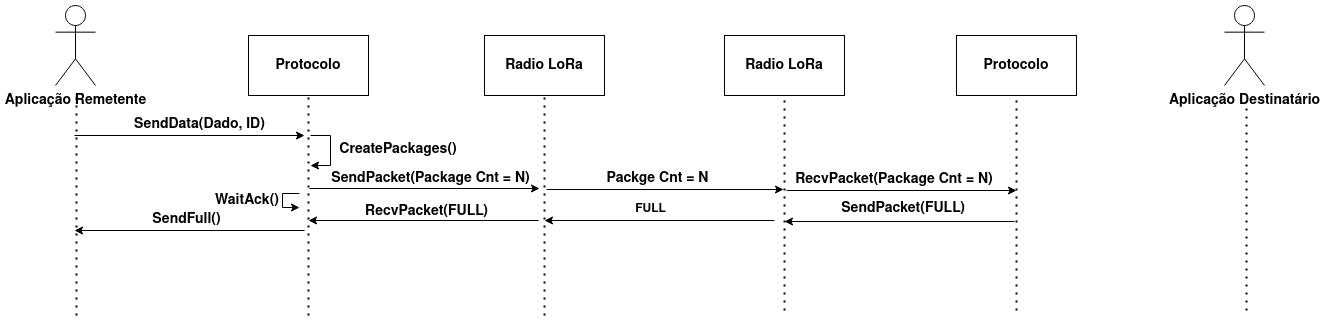
\includegraphics[width=\textwidth]{img/data-fa2.drawio.png}
    \label{fig:sq-data-fa2}
    Fonte: Autor, 2022.
\end{figure}

Diagrama baseado no caso de uso da tabela \ref{tab:use-cases05}.

\begin{figure}[htp]
    \centering
	\caption{Envio e Recebimento de Dados: Fluxo Alternativo 3}
    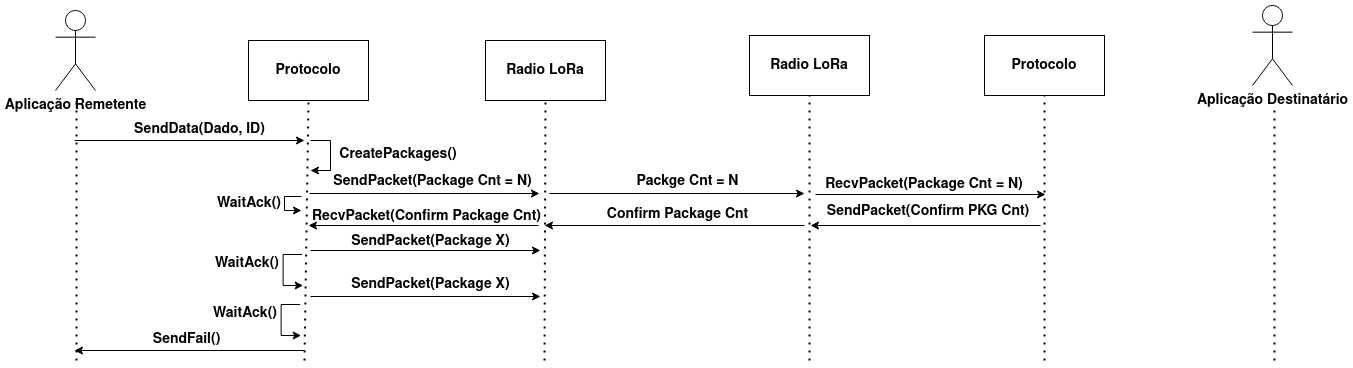
\includegraphics[width=\textwidth]{img/data-fa3.drawio.png}
    \label{fig:sq-data-fa3}
    Fonte: Autor, 2022.
\end{figure}

Diagrama baseado no caso de uso da tabela \ref{tab:use-cases05}.
\newpage

\begin{figure}[htp]
    \centering
	\caption{Envio e Recebimento de Dados: Fluxo Alternativo 4}
    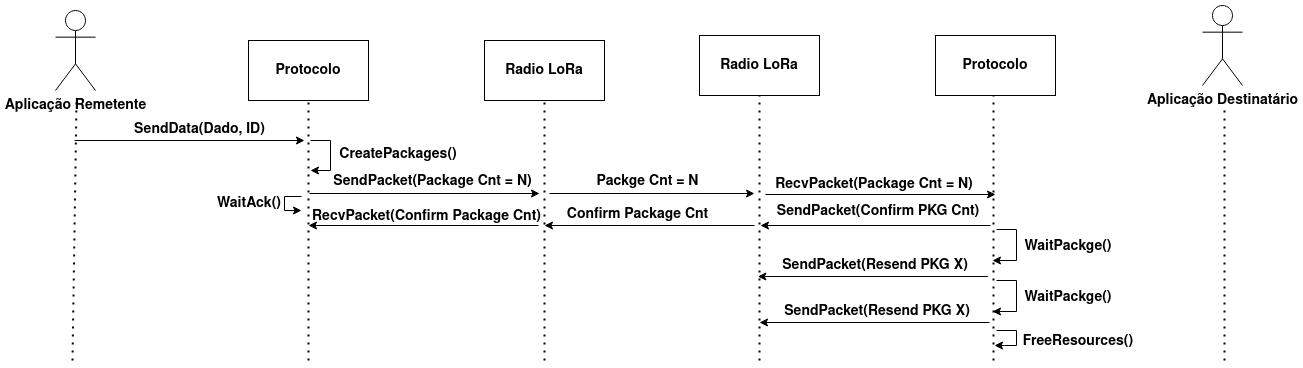
\includegraphics[width=\textwidth]{img/data-fa4.drawio.png}
    \label{fig:sq-data-fa4}
    Fonte: Autor, 2022.
\end{figure}

Diagrama baseado no caso de uso da tabela \ref{tab:use-cases05}.

\begin{figure}[htp]
    \centering
	\caption{Verificação de Atividade: Fluxo Normal}
    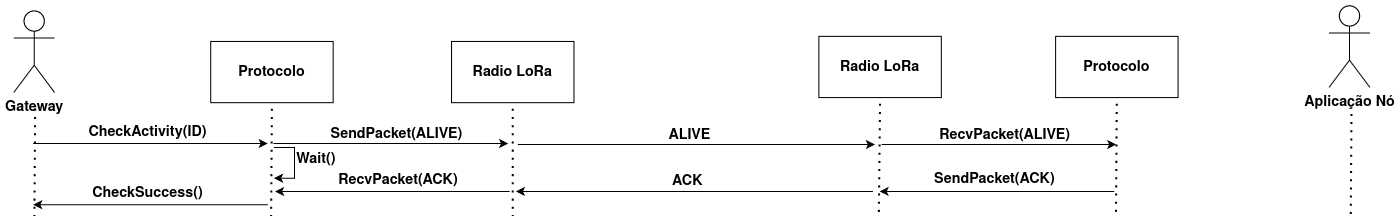
\includegraphics[width=\textwidth]{img/alive.drawio.png}
    \label{fig:sq-alive}
    Fonte: Autor, 2022.
\end{figure}

Diagrama baseado no caso de uso da tabela \ref{tab:use-cases06}.

\begin{figure}[htp]
    \centering
	\caption{Verificação de Atividade: Fluxo Alternativo}
    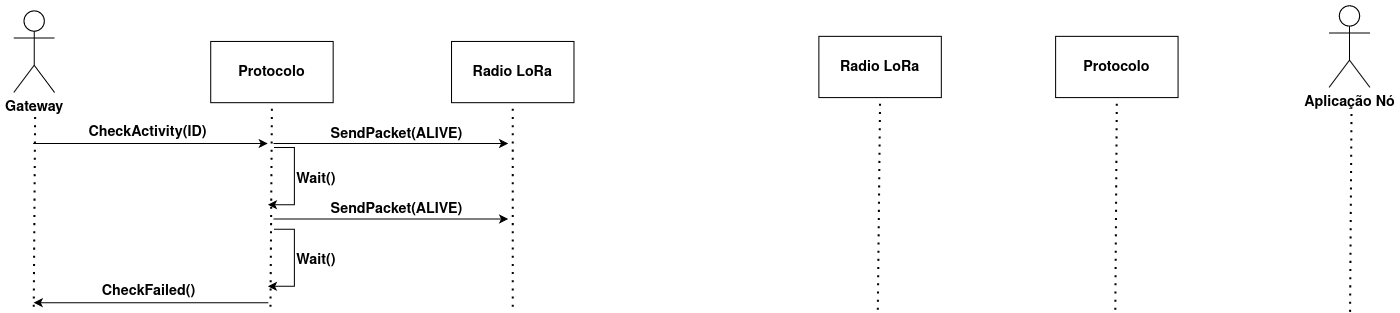
\includegraphics[width=\textwidth]{img/alive-fa.drawio.png}
    \label{fig:sq-alive-fa}
    Fonte: Autor, 2022.
\end{figure}

Diagrama baseado no caso de uso da tabela \ref{tab:use-cases06}.
\newpage

\subsection{Definição do Frame dos Pacotes}

Os diagramas de sequência ajudam a produzir uma etapa muito
importante do projeto que é importante a definição da
estrutura dos pacotes que vão estar trafegando pelos dispositivos da rede.
Dentro pacote é necessário o que chamamos de "metadados", que são
nada mais do que dados que contém informações sobre o pacote.
É graças aos metadados que as máquinas de estado, que serão criadas na próxima etapa,
podem entender que tipo de interação está acontecendo entre os módulos
naquele determinado estado, e dessa maneira, tomar ações. Pelo requisito
não-funcional \textbf{RNF02} os pacotes devem ter tamanho
máximo de até 256 bytes, o que nós da a quantidade de bytes que é preciso dividir
entre os metadados e os dados. Ainda pelos requisitos não-funcionais, o
requisito \textbf{RNF03} define que a Rede pode ter no máximo 255 dispositivos,
dessa forma é precisa no mínimo de 8 bits (1 byte) para identificar unicamente
todos os dispositivos da Rede. Levando essas informações em consideração, e
tomando como inspiração metadados de protocolos já existentes como o IP e MAC,
na figura \ref{fig:frame} e Tabela \ref{tab:metadata}, é apresentado a estrutura
do pacote definida para essa proposta.

\begin{figure}[htp]
    \centering
	\caption{Frame de um Pacote do Protocolo}
    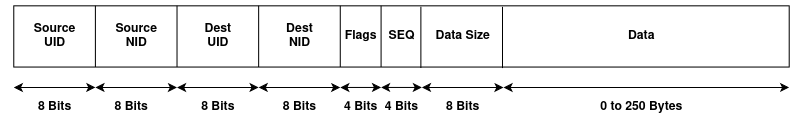
\includegraphics[width=\textwidth]{img/frame.drawio.png}
    \label{fig:frame}
    Fonte: Autor, 2022.
\end{figure}

\begin{longtable}{|l|l|}
    \caption{Detalhamento dos Metadados do Pacote}\label{tab:metadata}\\
    \hline
    Parâmetro & Descrição \\
    \hline
    Source UID & Identificador Único do Remetente \\
    \hline
    Source NID & Identificador de Rede do Remetente \\
    \hline
    Dest UID & Identificador Único do Destinatário \\
    \hline
    Dest NID & Identificador Rede do Destinatário \\
    \hline
    Flags & Tipo do Pacote \\
    \hline
    SEQ & Numero de sequência do Pacote \\
    \hline
    Data Size & Tamanho dos Dados \\
    \hline
\end{longtable}

Os conceitos de UID e NID são importantes pois, da mesma forma em que
um computador ao se conectar numa rede recebe um IP dinâmico do seu Modem, 
no protocolo proposto aqui, o Nó ao se conectar num Gateway receberá um
NID. Dessa forma o protocolo no Gateway pode gerenciar dinamicamente os
clientes da sua rede. Além de que, para o desenvolvedor da aplicação IoT,
o NID do seu dispositivo não importa, mas sim uma forma de poder identificar
um dispositivo especifico dentro da rede, para isso é usado o UID. O UID
é um identificador único restrito ao desenvolvedor, e através dele o desenvolvedor
pode solicitar ao protocolo para enviar dados para um UID especifico. Dessa
forma, os Rádios LoRa se comunicam por meio do NID, e as Aplicações por meio
do UID, um detalhe sútil mas que abre muitas possibilidades e flexibilidades.

\section{Documentação das Máquinas de Estado}

%Esta seção marca a última etapa da primeira fase, descrita anteriormente, de
%idealização e documentação. Ao final, teremos compreendido a problemática e
%produzido documentações baseadas na literatura que definem em alto nível o
%sistema proposto. \newline

A máquina de estado é uma das documentações que mais se aproxima de uma implementação
final. Numa máquina de estado definimos em que ponto se encontra o sistema (Estado
Atual), quais são as ações desse estado, e de que forma é possível de sair
de um estado para outros, além das ações que podem acontecer nas transições entre
estados. De certa formal, é possível visualizar máquinas de estado como
a tradução dos diagramas de sequência para uma lógica programável.

\subsection{Visão Geral}

Foram documentadas nessa proposta duas máquinas de estado, uma para o Gateway
e uma para o Nó. Apesar de distintas, as duas máquinas compartilham fluxos
comuns como o de envio e recebimento de dados, tornando possível construir
uma grande máquina única para os dois modos de operação. Porém, é importante
entender que, ao implementar em hardware, o protocolo em modo Gateway irá
requerer muito mais memória do que o protocolo em modo Cliente, isso se dá
pois o Gateway precisa gerenciar simultaneamente diferentes conexões com diferentes
clientes onde cada uma pode estar em estados distintos da máquina de estado.
Logo trará benefícios mais a frente no desenvolvimento a construção independente 
das máquinas de cada um.
Na Figura \ref{fig:node-fsm} e \ref{fig:gateway-fsm} podemos ter uma visão geral
das máquinas para o Nó e Gateway respectivamente. Nas sub-seções a frente
esse trabalho entrará em melhor detalhes de como os fluxos estão
implementados em cada uma. É importante ressaltar que cada fluxo detalhado foi
baseado nos diagramas de sequência produzidos na etapa anterior.

\clearpage

\begin{figure}[htp]
    \centering
	\caption{Visão Geral da Máquina de Estado do Nó}
    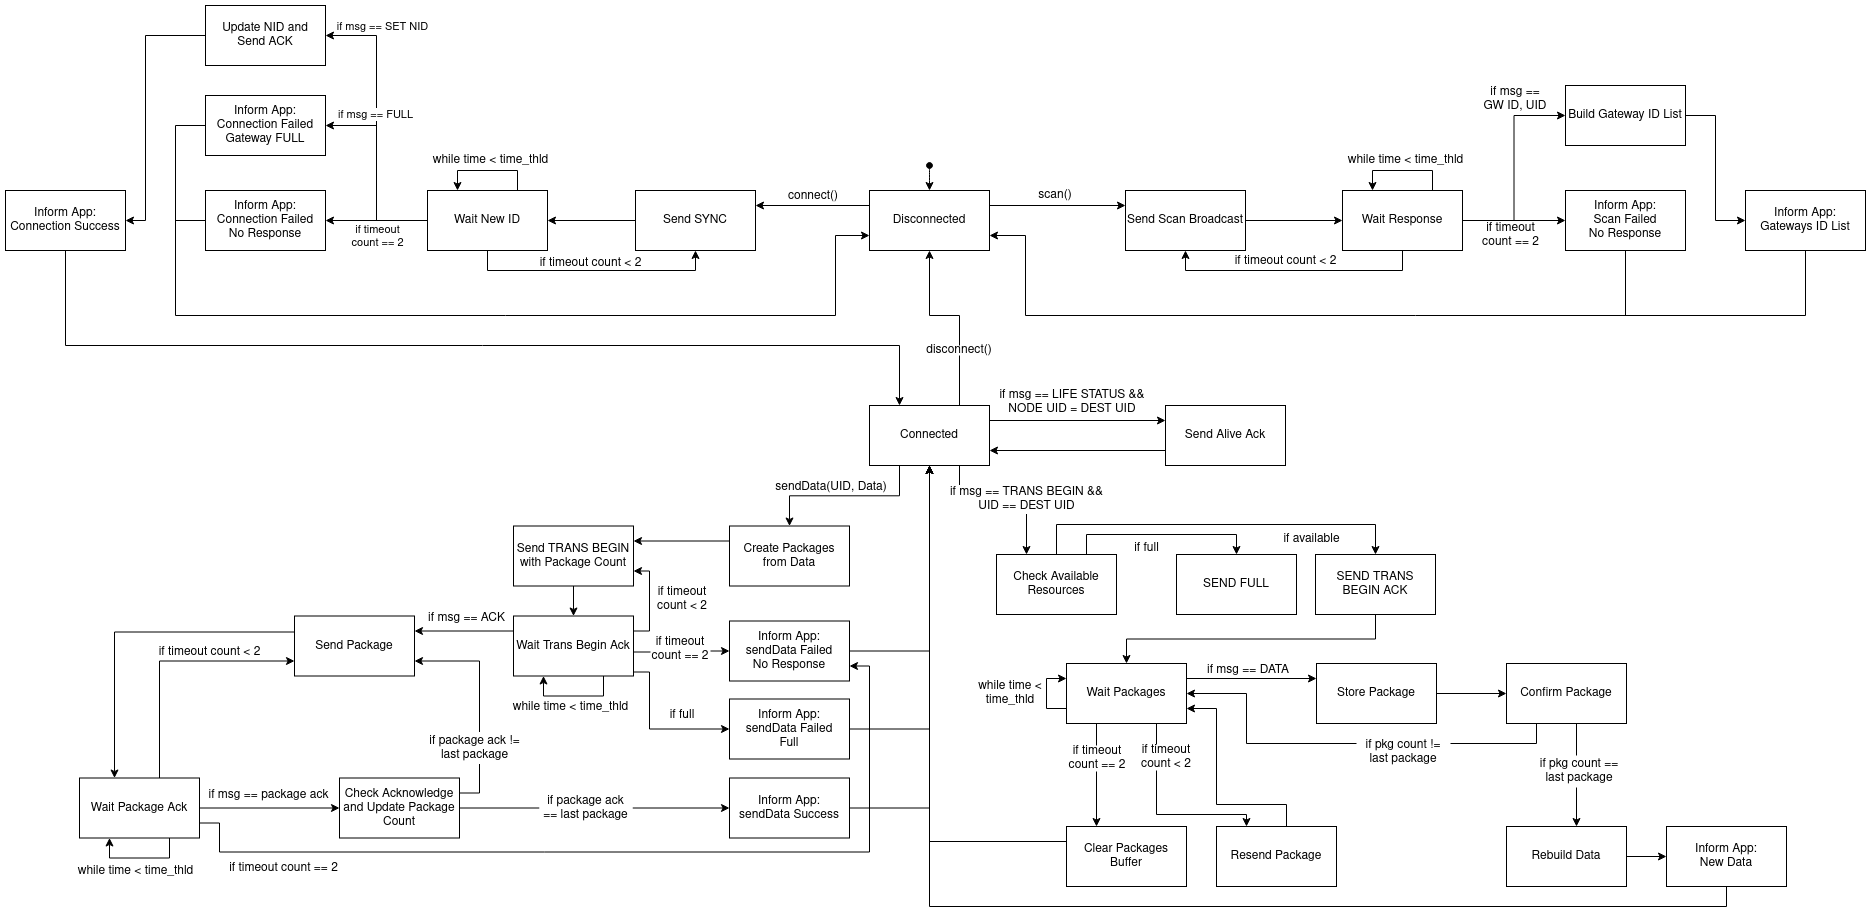
\includegraphics[width=\textwidth,height=0.3\textheight]{img/node_fsm.drawio.png}
    Fonte: Autor, 2022.
    \label{fig:node-fsm}
\end{figure}

\begin{figure}[htp]
    \centering
	\caption{Visão Geral da Máquina de Estado do Gateway}
    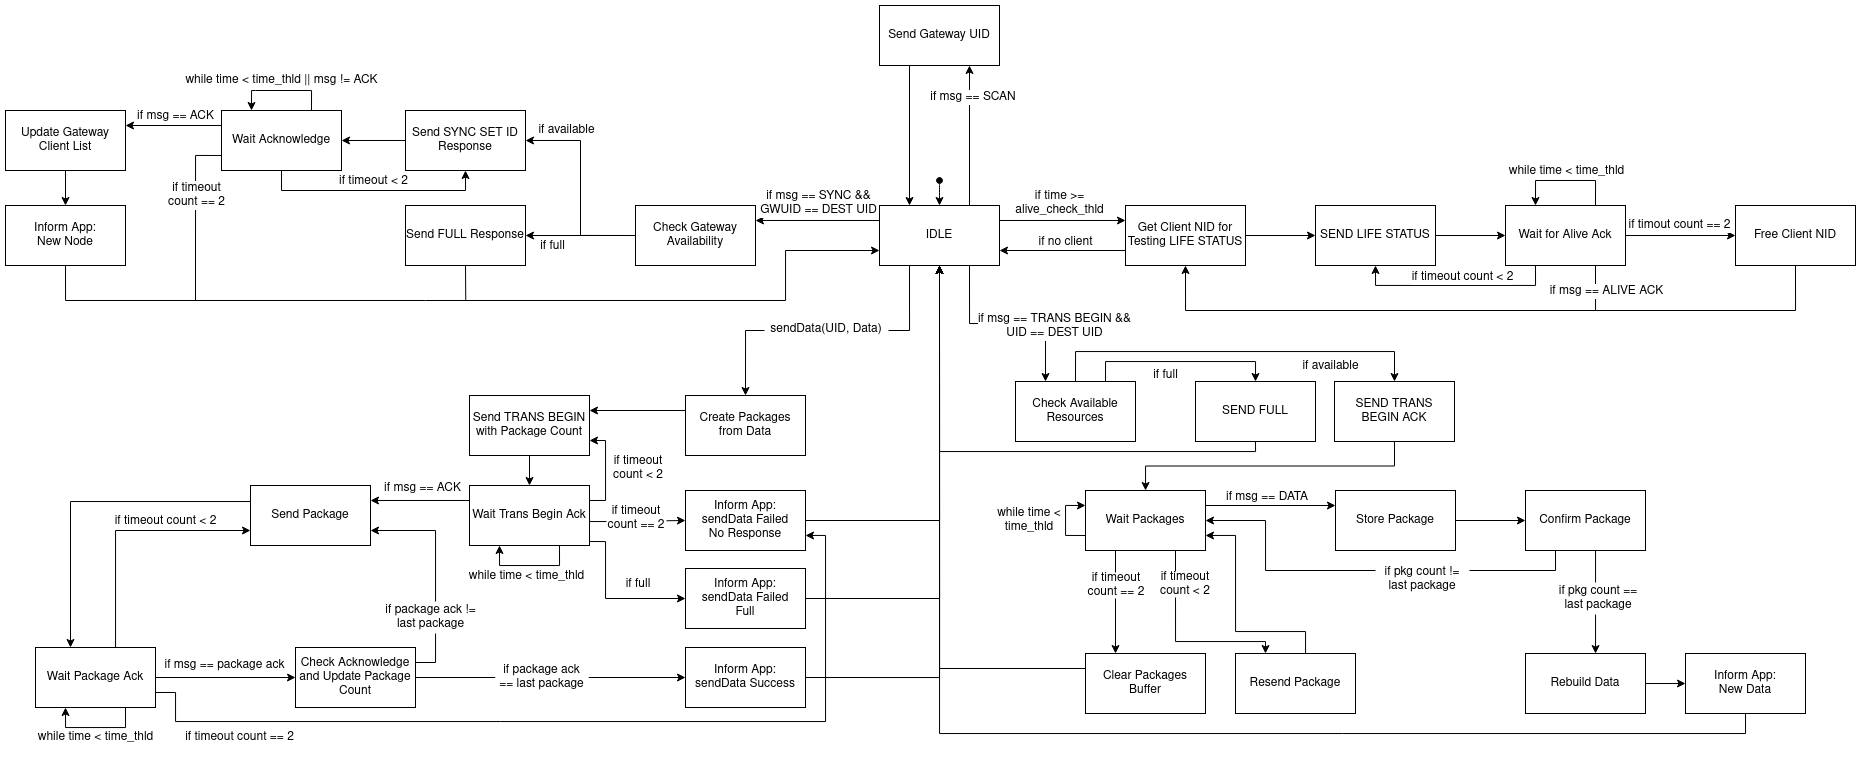
\includegraphics[width=\textwidth,height=0.315\textheight]{img/gateway_fsm.drawio.png}
    Fonte: Autor, 2022.
    \label{fig:gateway-fsm}
\end{figure}

\subsection{Estados de inicialização em Modo de Gateway ou Nó}

Esse fluxo é o mais simples de todos pois ele apenas configurará o
protocolo com o modo de operação devido e inicializará a maquina de estado
adequada. Logo ele não tem uma representação visual
nas máquinas de estado, mas, de certa forma, podem ser considerados
como o estado inicial delas.

\subsection{Estados de Varredura pelo Gateway}

Nesse fluxo, como pode ser visto nas figuras \ref{fig:fsm-node-scan} e \ref{fig:fsm-gw-scan},
o Nó se encontra em seu estado inicial de desconectado.
O objetivo é descobrir se existe algum Gateway na sua área de alcance,
então o Nó vai para o estado de enviar um sinal de varredura, e depois
para o estado de espera de uma resposta. Enquanto isso, um Gateway na
área de alcance e em seu estado inicial de espera recebe o sinal enviado
pelo Nó, logo esse passa para o estado de enviar uma resposta informando
o UID do Gateway presente na área, e depois volta para seu estado de espera
inicial. Ao Nó receber a resposta do Gateway, ele constrói uma lista
dcom o UID do Gateway e vai para o estado de informar a aplicação sobre
a varredura. Caso o Nó não receba nenhuma resposta dentro de um determinado
tempo após o envio do sinal de varredura, ele volta para o estado de envio
e tenta mais uma vez. Caso ainda sim não tenha uma resposta, ele vai para
o estado de informar a aplicação que a varredura não teve respostas.

\begin{figure}[htp]
    \centering
	\caption{Máquina De Estado do Nó: Varredura por Gateways}
    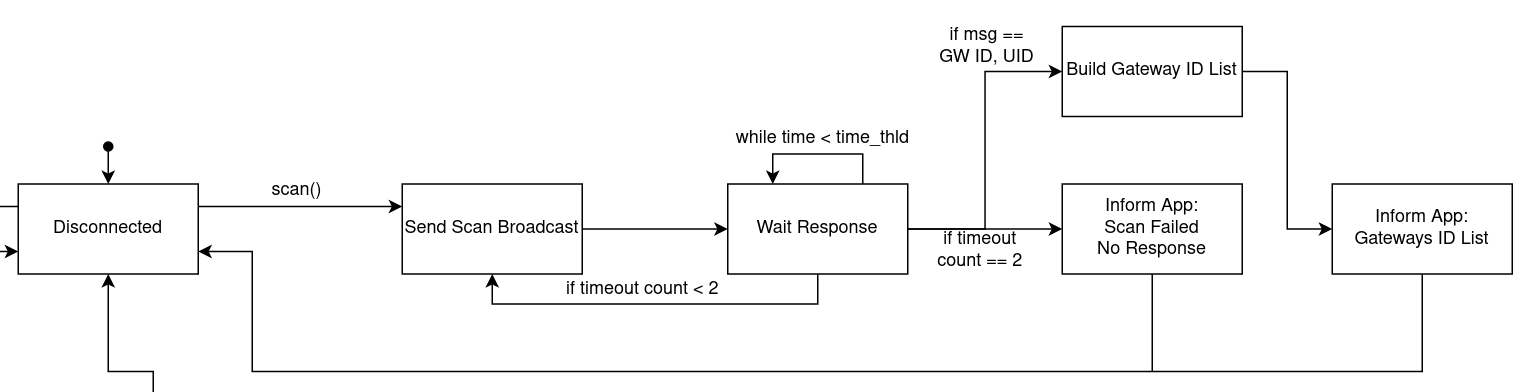
\includegraphics[width=\textwidth]{img/node-scan.drawio.png}
    Fonte: Autor, 2022.
    \label{fig:fsm-node-scan}
\end{figure}

\begin{figure}[htp]
    \centering
	\caption{Máquina De Estado do Gateway: Varredura por Gateways}
    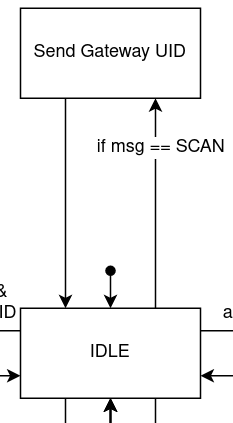
\includegraphics[width=0.15\textwidth]{img/gw-scan.drawio.png}
    
    Fonte: Autor, 2022.
    \label{fig:fsm-gw-scan}
\end{figure}

\subsection{Estados de Conexão com um Gateway}

Feita uma varredura para descobrir os UIDs de Gateways na área de alcance,
o Nó para se conectar vai para o estado de enviar uma sinal de sincronização
junto com o UID do Gateway que deseja conectar. Após o envio, o Nó vai para um
estado de espera por um determinado tempo. No Gateway, ao receber o sinal de sincronização,
é feito a troca de estado para verificar
se existe algum NID livre na Rede para reserva-lo ao Nó que solicitou a conexão.
Caso exista, o Gateway vai para o estado de responder ao Nó com um sinal de atualização para o novo NID
e logo em seguida fica no estado de aguardo da confirmação do Nó.
Caso não exista, ela vai para o estado de responder ao Nó que está com a
quantidade máxima de clientes e volta para o estado de espera. No Nó,
ao receber o sinal de atualização do novo NID, é feito a troca de estado para responder ao Gateway
com uma confirmação de que atualizou seu NID, depois para um estado
de informar a aplicação que a conexão foi bem sucedida e, por fim, o estado
de conectado. Caso o Nó receba o sinal de Gateway cheio, ele vai para
o estado que informa a aplicação que a conexão falhou pois o Gateway está
no limite máximo de clientes. Caso o Nó não receba nenhuma resposta do seu
pedido de sincronização dentro de um determinado tempo, ele volta para
o estado de conexão para tentar mais uma vez. Caso ainda sim, não tenha
resposta, o Nó vai para um estado de informar que a conexão falhou por
falta de resposta e volta para o seu estado de desconectado. Essa descrição pode ser vista nas
figuras \ref{fig:fsm-node-connect} e \ref{fig:fsm-gw-connect}.

\begin{figure}[htp]
    \centering
	\caption{Máquina De Estado do Nó: Conexão com um Gateway}
    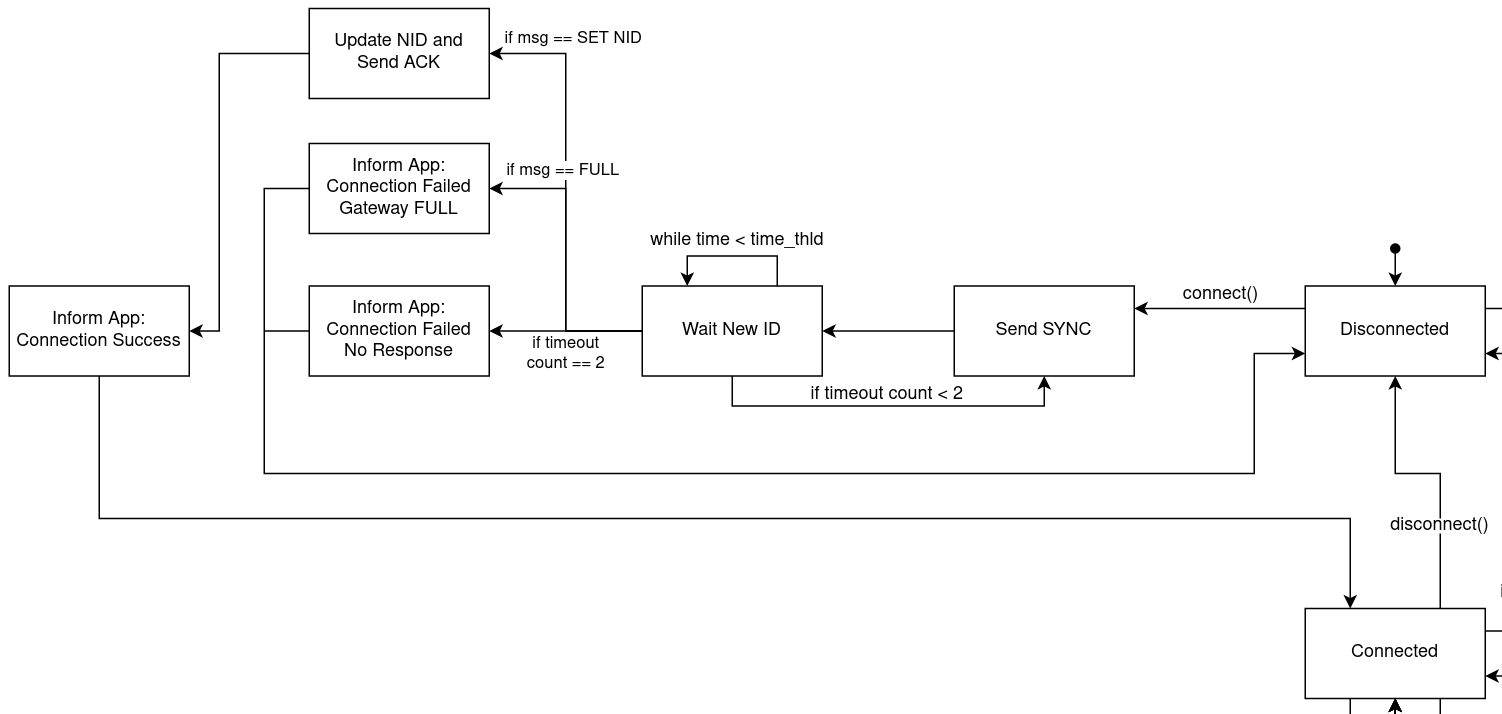
\includegraphics[width=\textwidth,height=0.32\textheight]{img/node-connect.drawio.png}
    Fonte: Autor, 2022.
    \label{fig:fsm-node-connect}
\end{figure}

\begin{figure}[htp]
    \centering
	\caption{Máquina De Estado do Gateway: Conexão com um Gateway}
    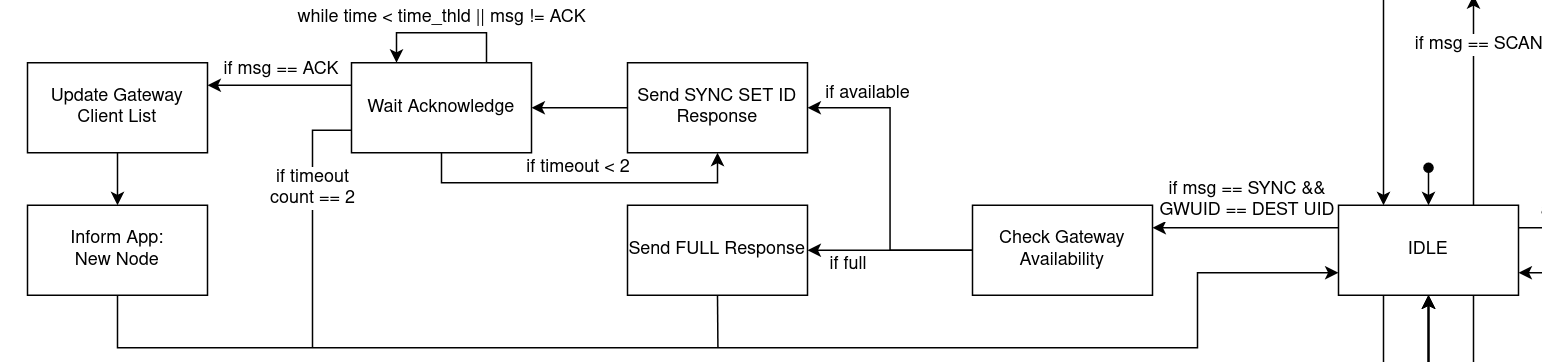
\includegraphics[width=\textwidth]{img/gw-connect.drawio.png}
    
    Fonte: Autor, 2022.
    \label{fig:fsm-gw-connect}
\end{figure}

\newpage

\subsection{Estados de Verificação de Atividade}

Quando um Nó se encontra num estado de conectado, seu UID está
incluso na lista de clientes do Gateways. De tempos em tempos
o Gateway faz uma verificação de atividade de todos seus clientes
para validar que ainda estão comunicáveis dentro da rede. O Gateway
vai para um estado de selecionar o UID do cliente a ser testado,
logo após vai para o estado de envio de sinal de atividade e, por fim,
o estado de espera de confirmação durante determinado tempo.
No Nó, ao estar no estado de conectado
e receber o sinal da verificação de atividade, ele vai para o estado
de resposta ao Gateway que continua comunicável dentro da rede.
Caso o Gateway não receba nenhuma resposta ao seu sinal, ele volta
para o estado de enviar sinal de atividade para tentar mais uma vez.
Caso ainda assim, ele não receba nenhuma resposta, ele vai para o
estado de remoção do NID da lista de clientes, e a partir desse estado
o NID está agora livre para uso em outro cliente que solicitar uma
conexão. Após esse estado, o Gateway volta para o estado de selecionar
um cliente a ser testado, até que não tenha mais nenhum cliente a
testar, logo ele volta pra o estado de espera.

\begin{figure}[htp]
    \centering
	\caption{Máquina De Estado do Nó: Verificação de Atividade}
    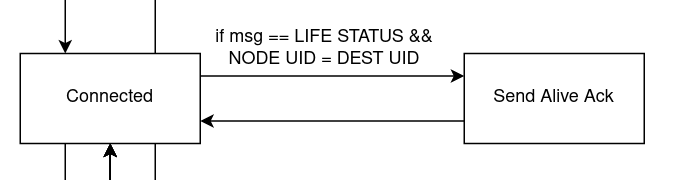
\includegraphics[width=0.6\textwidth]{img/node-alive.drawio.png}
    
    Fonte: Autor, 2022.
    \label{fig:fsm-node-alive}
\end{figure}

\begin{figure}[htp]
    \centering
	\caption{Máquina De Estado do Gateway: Verificação de Atividade}
    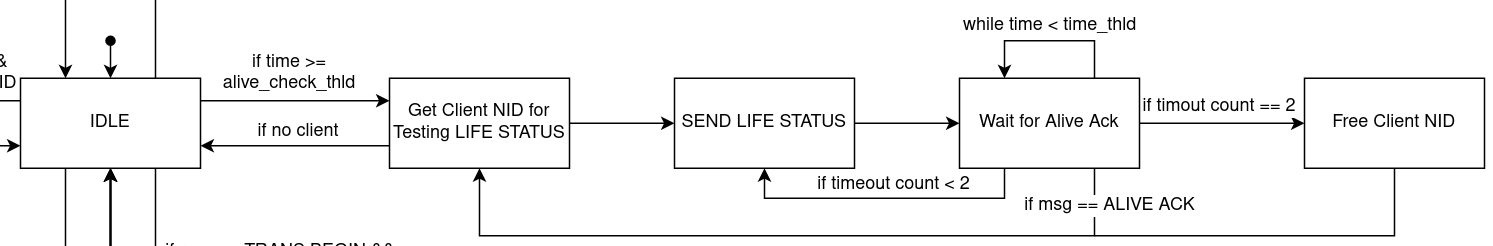
\includegraphics[width=\textwidth]{img/gw-alive.drawio.png}
    
    Fonte: Autor, 2022.
    \label{fig:fsm-gw-alive}
\end{figure}

\subsection{Estados de Envio e Recebimento de Dados}

Os estados de envio e recebimento de dados são comuns para as duas máquinas
implementadas nessa seção. Assim, o fluxo é o mesmo seja um envio do Nó ao
Gateway como do Gateway para o Nó. Ao inciar um fluxo de envio de dados para
um UID especifico, o remetente vai para um estado de dividir os dados em N
pacotes e logo após para o estado de informar o destinatário que deseja fazer
uma transmissão, quantos pacotes pretende enviar, e fica no estado de aguardo.
O destinatário permanece no estado de aguardo até que receba alguma resposta ou
que tenha tentado solicitar a transmissão num total de 2 vezes e mesmo assim não
obteve uma resposta. Já no remetente, ao receber o sinal de solicitação de transmissão,
é feito a mudança para o estado de verificar se existe recursos disponíveis para aceitar
a transmissão, caso sim, é enviado um sinal aceitando a transmissão, caso não, é enviado
um sinal informando que não será possível. A partir desse ponto, tanto o remetente e o
destinatário estão sincronizados para a transmissão, a logica a seguir é, ao envio de cada
pacote, o destinatário precisa acusar o recebimento, caso o recebimento não seja confirmado
o remetente reenvia o mesmo pacote mais uma vez, e se mesmo assim não for confirmado, ele
desistirá da transmissão. Já o destinatário fica no aguardo do pacote com o numero de sequencia
correto, caso ele não receba, ele solicita ao remetente o reenvio desse pacote, se ainda sim ele
não receber, ele desistirá da transmissão. Ao final da transmissão bem sucedida, o destinatário
segue para o estado de reconstrução do dados a partir dos pacotes recebidos e em seguida informa
a aplicação a existência de dados recém chegados.

\begin{figure}[htp]
    \centering
	\caption{Máquina De Estado do Nó: Envio e Recebimento de Dados}
    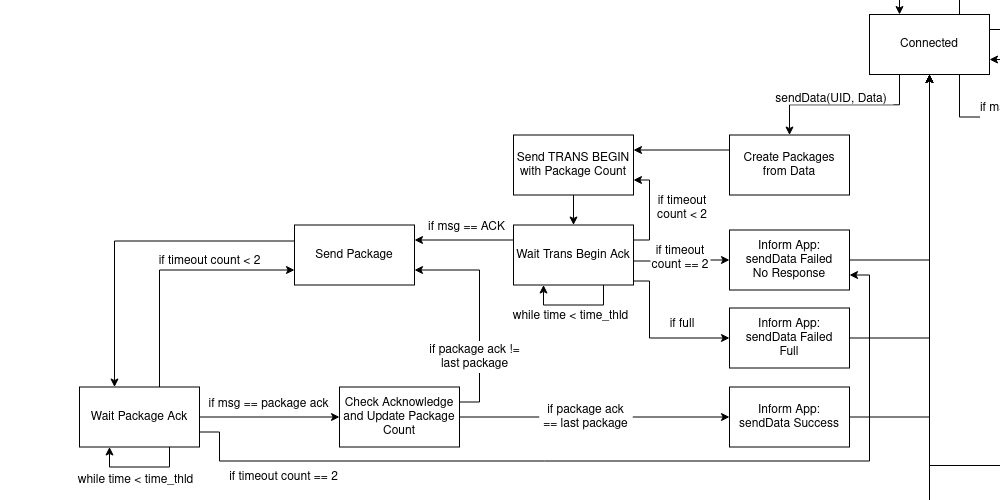
\includegraphics[height=0.27\textheight,keepaspectratio]{img/node-send.drawio.png}
    
    Fonte: Autor, 2022.
    \label{fig:fsm-node-send}
\end{figure}

\begin{figure}[htp]
    \centering
	\caption{Máquina De Estado do Gateway: Envio e Recebimento de Dados}
    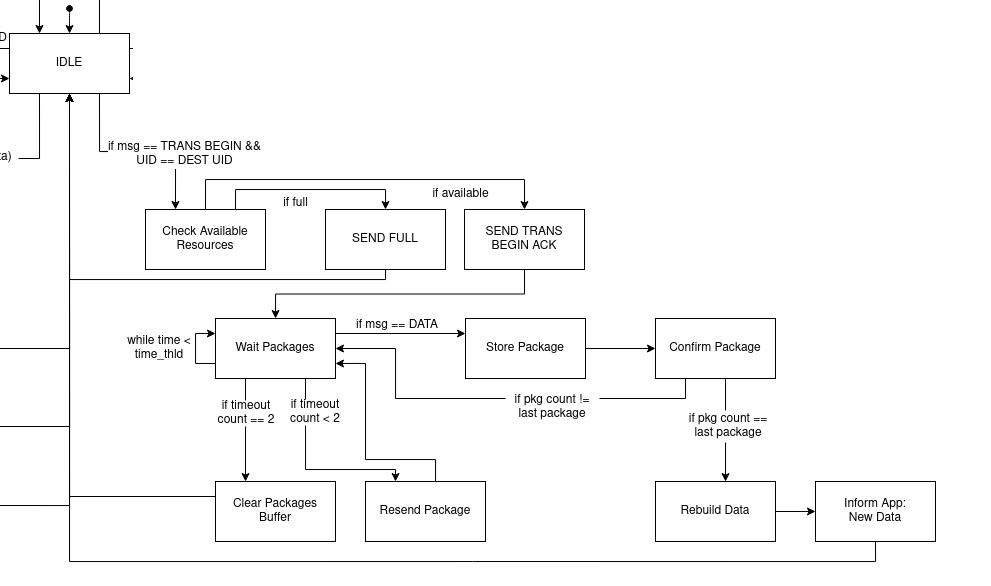
\includegraphics[height=0.28\textheight,keepaspectratio]{img/gw-recv.drawio.png}
    
    Fonte: Autor, 2022.
    \label{fig:fsm-gw-recv}
\end{figure}

\clearpage

\section{Implementação da Arquitetura e Abstração do Hardware}

Esta etapa tem o objetivo de usar de toda documentação gerada na primeira fase
e implementá-la em código executável. Nessa etapa vamos nós preocupar em entender
como o hardware funciona, desde o rádio LoRa aos possíveis microcontroladores, e
as funcionalidades oferecidas por eles e necessárias para a implementação real
da proposta. Para garantir uma boa qualidade de software com códigos bem estruturados
e reutilizáveis, é importante definir um diagrama de blocos da Arquitetura, por meio
do diagrama é possível ver os módulos de software como caixas pretas, a forma que
eles se interagem, os recursos que precisam, e a sua plataforma, que no caso dessa
proposta é o dispositivo embarcado do desenvolvedor IoT. É importante frisar que por
questão de portabilidade, o diagrama representa uma especificação genérica dos softwares
e funcionalidades que podem ser encontradas em vários tipos de dispositivos embarcados,
isso é importante pois garante de certo nível teórico que o protocolo pode ser implementado
apenas uma vez e portado para vários dispositivos.

\subsection{Diagrama de Blocos}

\begin{figure}[h]
    \centering
	\caption{Diagrama macro do Hardware e Software}
    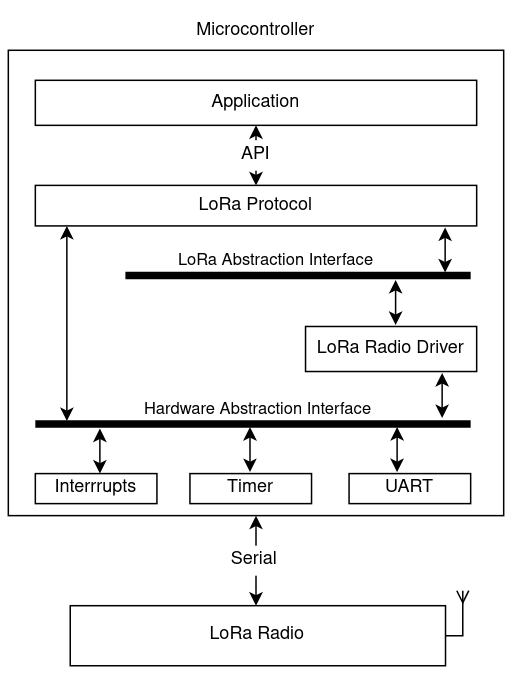
\includegraphics[width=0.5\textwidth,height=0.5\textheight,keepaspectratio]{img/blk.drawio.png}
    \label{fig:blk}
    
    Fonte: Autor, 2022.
\end{figure}

O Diagrama de Blocos definido na Figura \ref{fig:blk} representa a estrutura de software
definida para esse trabalho. A aplicação conversa com o protocolo por meio de uma API
(Application Progamming Interface) que por sua vez utiliza recursos do hardware por
meio de camadas de abstração, chamadas de \textit{Interfaces}, que por sua vez chamam 
as funções específicas do hardware a ser utilizado.
Dessa forma, mesmo que o hardware e/ou rádio LoRa mudem, não é necessário refatorar
nenhuma parte do código do protocolo. Nas próximas sub-seção será melhor descrito como
foi atingida essa abstração nesse trabalho.

\subsection{Módulos internos do Protocolo}

O protocolo possui 5 componentes extremamente importantes para garantir uma boa modularização,
uma boa utilização dos recursos de hardware, e mais importante ainda, garantir todas as funcionalidades
descritas nas documentações, nessa sub-seção vamos entrar em detalhes sobre esses componentes. Na
figura \ref{fig:gw-blk} a seguir é possível visualizar esses 5 módulos que compõe o módulo final do
Gateway.

\begin{figure}[H]
    \centering
	\caption{Diagrama micro do modulo do protocolo para o Gateway}
    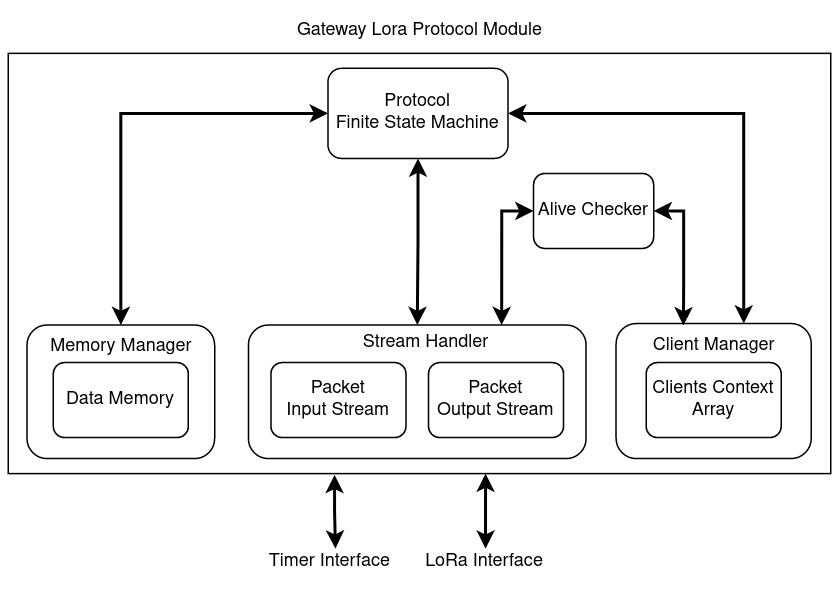
\includegraphics[height=0.3\textheight,keepaspectratio]{img/gw-block.drawio.png}
    \label{fig:gw-blk}
    
    Fonte: Autor, 2022.
\end{figure}

\subsubsection{Stream Handler}

O stream handler é um modulo para gerenciar os pacotes que estão indo e vindo pelo protocolo,
ele possui duas filas circulares, uma para os pacotes de entrada, e uma para os pacotes de saída,
sua função principal é de ordenar a ordem de tratamento dos pacotes e servir como um buffer temporário
enquanto a maquina de estado estiver ocupada. Na figura \ref{fig:code-sh} é possível ver a implementação
do modulo.

\begin{figure}[H]
    \centering
	\caption{Código do Stream Handler}
    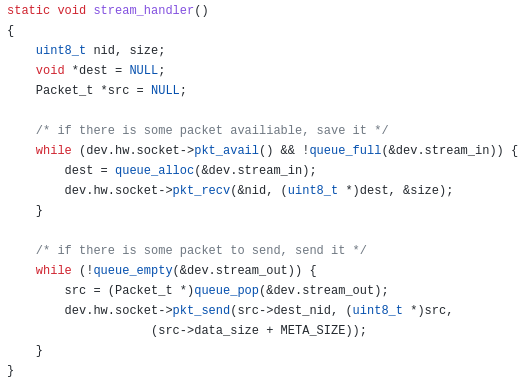
\includegraphics[height=0.3\textheight,keepaspectratio]{img/stream-handler.png}
    \label{fig:code-sh}
    
    Fonte: Autor, 2022.
\end{figure}

\subsubsection{Client Manager}

O client manager é um conjunto de APIs usadas pela maquina de estado e pelo modulo de Alive Checker
para interagir com uma área de memoria responsável por guardar informações criticas para cada conexão,
essa área de memoria é um array com indexação baseada no NID do cliente. Na figura \ref{fig:code-clt-ctx} a seguir é possível ver os dados armazenados para cada entrada desse array.

\begin{figure}[H]
    \centering
	\caption{Dados de uma entrada do array de clientes}
    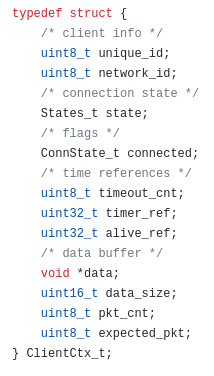
\includegraphics[height=0.3\textheight,keepaspectratio]{img/clt-ctx.png}
    \label{fig:code-clt-ctx}
    
    Fonte: Autor, 2022.
\end{figure}

\subsubsection{Alive Checker}

O alive checker é o modulo responsável por estar sempre analisando a lista de clientes e
validando a se algum cliente passou muito tempo sem se comunicar, dependendo do tempo limite
configurado, ele testará cada cliente que passar desse limiar. Na figura \ref{fig:code-alive-checker} a seguir é possível ver sua implementação.

\begin{figure}[H]
    \centering
	\caption{Código do Alive Checker}
    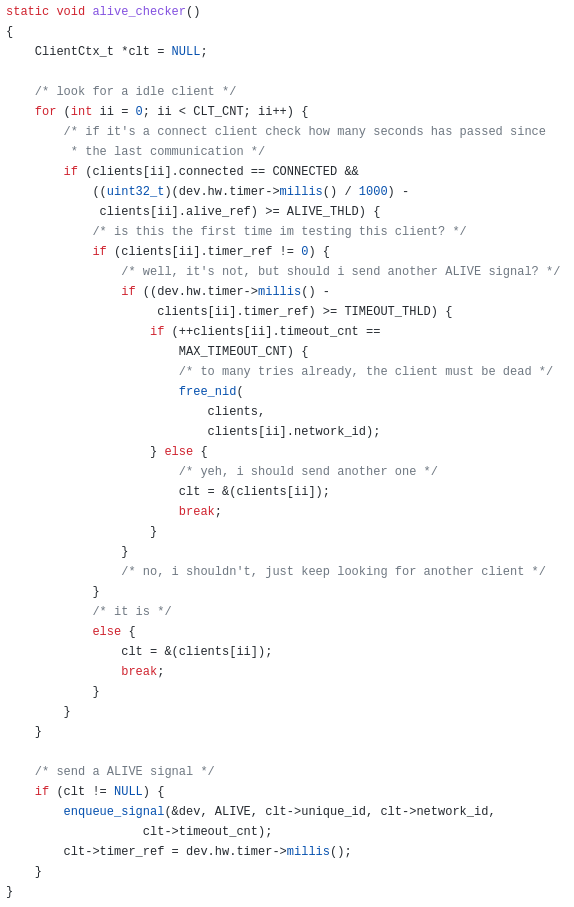
\includegraphics[height=0.7\textheight,keepaspectratio]{img/alive-checker.png}
    \label{fig:code-alive-checker}
    
    Fonte: Autor, 2022.
\end{figure}

\subsubsection{Memory Manager}

o memory manager é o modulo que implementa algoritmos de alocação dinâmica de um determinado espaço
continuo de memoria. O memory manager é um modulo extramente pois é a partir dele que o Gateway consegue
ter diferentes espaços de memoria reservados para as diferentes transmissões de dados simultâneas que possam acontecer. Com isso é possível garantir que o protocolo use uma quantidade especifica de memoria do hardware mas que será gerenciada de maneira inteligente para diferentes recursos. Na figura \ref{fig:code-memmgr-api} a seguir é possível ver as APIs do memory manager.

\begin{figure}[H]
    \centering
	\caption{APIs do Memory Manager}
    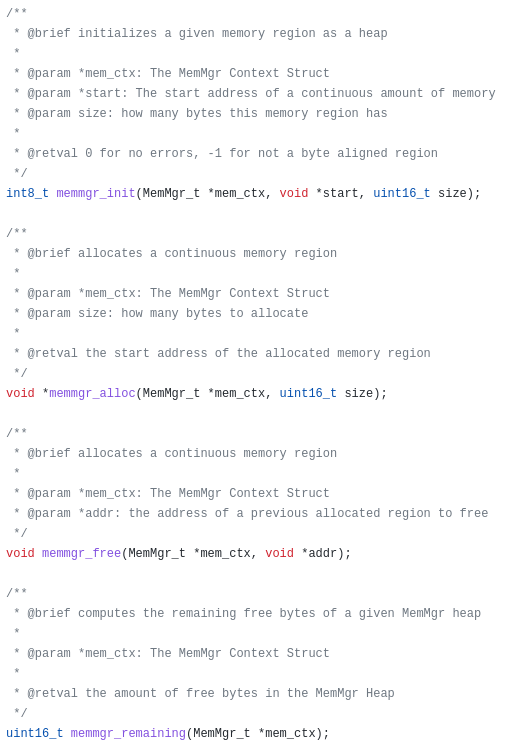
\includegraphics[height=0.55\textheight,keepaspectratio]{img/memmgr-api.png}
    \label{fig:code-memmgr-api}
    
    Fonte: Autor, 2022.
\end{figure}

\subsubsection{Protocol Finite State Machine}

A maquina de estado implementada é o maior modulo em relação a linhas de código, ela que
garantes as funcionalidades e fluxos definidos nas etapas de documentação. Sua implementação
é a tradução direta para código do que foi documento na etapa de geração das maquinas de estado.

\subsubsection{Juntando os componentes}

Com isso, o modulo macro do procolo foi definido numa estrutura que pode ser vista na figura \ref{fig:dev}
e sua inicialização na figura \ref{fig:gw-init}.

\begin{figure}[H]
    \centering
	\caption{Estrutura do protocolo macro}
    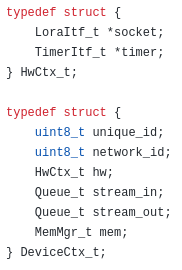
\includegraphics[height=0.2\textheight,keepaspectratio]{img/dev.png}
    \label{fig:dev}
    
    Fonte: Autor, 2022.
\end{figure}

\begin{figure}[H]
    \centering
	\caption{Inicialização da estrutura do protocolo macro}
    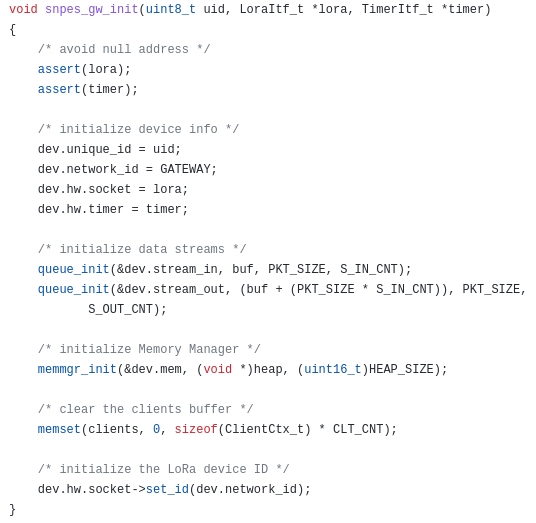
\includegraphics[height=0.4\textheight,keepaspectratio]{img/gw-init.png}
    \label{fig:gw-init}
    
    Fonte: Autor, 2022.
\end{figure}

\subsection{Removendo as dependências do Hardware}

No geral, recursos de hardware, seja qual for a arquitetura, são acessados
por meio de leituras e escritas em endereços de memória específicos. Esses
endereços recebem uma nomenclatura especial de \textit{Registradores}. De maneira
simples, um programador que deseja mudar o estado de um pino numa porta
GPIO entre HIGH e LOW, basta mudar o bit que representa o pino
de interesse no registrador da porta GPIO. Apesar da teoria ser a mesma
para muitos casos de microcontroladores, a pratica não é, pois os registradores
diferem de estrutura e endereço de arquitetura para arquitetura.

Isso implica que, ao desenvolver alguma funcionalidade que utilize recursos
do hardware, ela teria que ser rescrita para cada arquitetura final, algo
totalmente impraticável se o objetivo é suportar diferentes hardwares. Como
solução para esse problema surgiu o conceitos de \textit{Interfaces}

\subsubsection{Abstração com Interfaces}

Interfaces é um conceito extramente usado no kernel Linux, em outros sistemas
operacionais e firmwares para obter abstração e modularização. Uma interface
é simplesmente uma \textbf{estrutura} que \textbf{descreve} funcionalidades. Por exemplo,
uma transmissão serial possui as \textbf{funcionalidades} de \textit{escrever}
e \textit{ler} bytes por um determinado canal, funções mais alto nível que desejam
utilizar essas funcionalidades podem ter como \textbf{dependência} a interface
que as definem. Dessa forma, é possível que para cada mudança de hardware
seja apenas necessário atualizar quais funções especificas essa interface apontará,
e com isso nenhuma mudança de código será necessária já que as funções mais alto
nível \textbf{dependem} da interface e sua definição nunca muda. Nas figuras
\ref{fig:itf-timer} e \ref{fig:itf-lora} a seguir é possui visualizar em código as interfaces
definidas nesse projeto para as funcionalidades de Timer e Rádio loRa respectivamente.

\begin{figure}[H]
    \centering
	\caption{Interface Timer}
    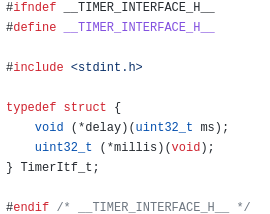
\includegraphics[height=0.19\textheight,keepaspectratio]{img/itf-timer.png}
    \label{fig:itf-timer}
    
    Fonte: Autor, 2022.
\end{figure}

\begin{figure}[H]
    \centering
	\caption{Interface LoRa}
    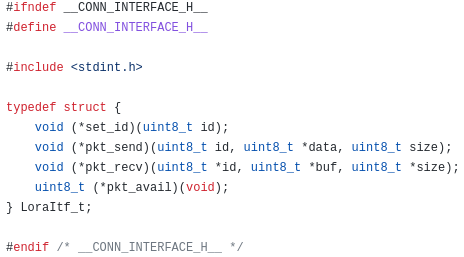
\includegraphics[height=0.2\textheight,keepaspectratio]{img/itf-lora.png}
    \label{fig:itf-lora}
    
    Fonte: Autor, 2022.
\end{figure}

\newpage

Pelas figuras é possível ver que as interfaces são simplesmente um conjunto
de ponteiros que direcionam para as funções dependentes do hardware. Na figura
\ref{fig:gw-init-def} a seguir é possível visualizar que o protocolo depende dessas interfaces.
E nas figuras \ref{fig:timer-ex} e \ref{fig:lora-ex} é possível visualizar
exemplos de uso dessas interfaces.

\begin{figure}[H]
    \centering
	\caption{Assinatura de função de inicialização do Protocolo}
    \includegraphics[height=0.14\textheight,keepaspectratio]{img/gw-init-def.png}
    \label{fig:gw-init-def}
    
    Fonte: Autor, 2022.
\end{figure}

\begin{figure}[H]
    \centering
	\caption{Exemplo de uso da Interface Timer}
    \includegraphics[width=0.7\textwidth,keepaspectratio]{img/timer-ex.png}
    \label{fig:timer-ex}
    
    Fonte: Autor, 2022.
\end{figure}

\begin{figure}[H]
    \centering
	\caption{Exemplo de uso da Interface LoRa}
    \includegraphics[height=0.09\textheight,keepaspectratio]{img/lora-ex.png}
    \label{fig:lora-ex}
    
    Fonte: Autor, 2022.
\end{figure}

\newpage

\subsection{Implementação final}

A implementação final do projeto ficou de acordo com a tabela \ref{tab:files} a seguir
e pode ser publicamente acessada na url: \url{https://github.com/mfbsouza/snpes}. O projeto
final ganhou o apelido de "SNPES" [isnepis] que significa Simple Network Protocol for Embedded
Systems.  

\begin{longtable}{|l|l|l|}
    \caption{Arquivos de código do Projeto}\label{tab:files}\\
    \hline
    \textbf{Pasta} & \
    \textbf{Arquivo} & \
    \textbf{Qnt. de linhas} \\
    \cline{1-3}
    src & \
    CircularQueue.c & \
    123 \\
    \cline{2-3}
     & \
    CircularQueue.h & \
    90 \\
    \cline{2-3}
     & \
    ConnInterface.h & \
    13 \\
    \cline{2-3}
     & \
    MemoryManager.c & \
    113 \\
    \cline{2-3}
     & \
    MemoryManager.h & \
    60 \\
    \cline{2-3}
     & \
    snpes\_cfg.h & \
    49 \\
    \cline{2-3}
     & \
    snpes\_gateway.c & \
    351 \\
    \cline{2-3}
     & \
    snpes\_gateway.h & \
    49 \\
    \cline{2-3}
     & \
    snpes\_node.c & \
    186 \\
    \cline{2-3}
     & \
    snpes\_node.h & \
    55 \\
    \cline{2-3}
     & \
    snpes\_types.h & \
    88 \\
    \cline{2-3}
     & \
    snpes\_utils.c & \
    128 \\
    \cline{2-3}
     & \
    snpes\_utils.h & \
    122 \\
    \cline{2-3}
     & \
    TimerInterface.h & \
    11 \\
    \hline
    
    tests & \
    AllTests.cpp & \
    6 \\
    \cline{2-3}
     & \
    CircularQueueTests.cpp & \
    166 \\
    \cline{2-3}
     & \
    MemoryManagerTests.cpp & \
    117 \\
    \cline{2-3}
     & \
    SnpesGatewayTests.cpp & \
    532 \\
    \cline{2-3}
     & \
    SnpesNodeTests.cpp & \
    248 \\
    \cline{2-3}
     & \
    SnpesUtilsTests.cpp & \
    150 \\
    \hline
    
    Total & \
     & \
    2657 \\
    \hline
\end{longtable}
\chapter{Validação e Resultados}

Nesse capítulo será apresentado o processo de validação e análise do projeto
desenvolvido nessa proposta. A validação foi divida em 2 etapas, a primeira
foi a validação via software, por meio de simulações e ferramentas de teste,
e a segunda foi a validação via hardware, onde foi produzido sistemas embarcados
protótipos para teste do protocolo no mundo real. Nas seções a seguir esse
trabalho irá entrar detalhes no que foi feito em cada etapa e quais foram
os resultados obtidos.

\section{Simulações e Testes Unitários}

O desenvolvimento dos códigos desse projeto seguiu a metodologia \textit{Test Driven Development}
a qual determina que a medida em que os módulos de um sistema vão sendo desenvolvidos, é desenvolvido
em paralelo também as suas próprias rotinas de testes. Tais testes podem ser divididos em categorias
como \textit{teste de integração}, onde é testado a integração entre diferentes módulos, e como o
\textit{teste unitário}, onde é testado o modulo como um caixa preta fora do sistema. Pare isso,
existem hoje em dia várias \textit{frameworks} que ajudam o desenvolvedor nesse processo,
nesse trabalho foi utilizada a framework \textit{CppUTest}, uma framework voltada para
testes unitários em projetos de sistemas embarcados.

Um teste unitário é nada mais do que rotinas de testes que são escritas em código e que
interagem com os módulos desenvolvidos e testam se, dependendo da entrada, foi produzido
a saída esperada. Nas figuras \ref{fig:test-queue} e \ref{fig:test-memmgr} a seguir é possível
visualizar exemplos dessas rotinas de testes.

\begin{figure}[H]
    \centering
	\caption{Teste das funcionalidades do modulo Circular Queue}
    \includegraphics[height=0.75\textheight,keepaspectratio]{img/test-queue.png}
    \label{fig:test-queue}
    
    Fonte: Autor, 2022.
\end{figure}

\begin{figure}[H]
    \centering
	\caption{Teste das funcionalidades de alocação do modulo Memory Manager}
    \includegraphics[height=0.62\textheight,keepaspectratio]{img/test-memmgr.png}
    \label{fig:test-memmgr}
    
    Fonte: Autor, 2022.
\end{figure}

\subsection{Testes Unitários como Simuladores}

Uma possibilidade que os testes unitários fornecem é a de simular fluxos do protocolo.
Ao ver todo o modulo do projeto como uma caixa preta, podemos entender que na
sua entrada vamos ter diferentes tipos de pacotes que serão processados seguindo
alguma lógica definida internamente e na sua saída um outro pacote como resposta deste
estimulo de entrada. Seguindo essa logica, foi desenvolvido testes para cada fluxo
proposto nesse projeto. Na figura \ref{fig:test-gw} a seguir podemos ver uma trecho
de um dos testes para validar o fluxo de conexão com o gateway.

\begin{figure}[H]
    \centering
	\caption{Teste de fluxo de conexão de nó com gateway}
    \includegraphics[width=0.75\textwidth,keepaspectratio]{img/test-gw.png}
    \label{fig:test-gw}
    
    Fonte: Autor, 2022.
\end{figure}

\subsection{Resultado dos Testes Unitários}

Foram desenvolvidas 41 rotinas de testes totalizando 525 verificações afim
de validar todos as funcionalidades de cada modulo do sistema como também
simular o sistema como um todo para todos os fluxos propostos nesse trabalho.
É interessante observar que, como mostra na figura \ref{fig:langs} a seguir
e também na tabela \ref{tab:files}, aproximadamente metade de todo código 
produzido no projeto foi para testes, que foram exclusivamente escritos em C++.

\begin{figure}[H]
    \centering
	\caption{Percentual das linguagens presentes no projeto}
    \includegraphics[height=0.11\textheight,keepaspectratio]{img/langs.png}
    \label{fig:langs}
    
    Fonte: Autor, 2022.
\end{figure}

Na figura \ref{fig:tests} a seguir é possível ver o resultado dos testes desenvolvidos,
onde todos passaram com sucesso.

\begin{figure}[H]
    \centering
	\caption{Execução dos testes desenvolvidos}
    \includegraphics[height=0.57\textheight,keepaspectratio]{img/tests.png}
    \label{fig:tests}
    
    Fonte: Autor, 2022.
\end{figure}

\newpage

\subsection{Cobertura do código}

Além das APIs de testes, a framework \textit{CppUTest} oferece a geração de
\textit{relatórios de cobertura}. Esses relatórios descrevem a porcentagem de
linhas de código de cada arquivo fonte que foram testadas. Além disso ele
gera também um descrição de quantas vezes qualquer linha de código do projeto
foi executada e quais não foram. Na figura \ref{fig:cov} a seguir é possível
visualizar o resultado de cobertura do projeto.

\begin{figure}[H]
    \centering
	\caption{Relatório de cobertura do projeto}
    \includegraphics[height=0.225\textheight,keepaspectratio]{img/cov.png}
    \label{fig:cov}
    
    Fonte: Autor, 2023.
\end{figure}

Como é visto na figura a cima o projeto teve 100\% de cobertura no código,
ou seja, todas as linhas programadas foram executadas pelo menos uma vez.

\section{Protótipos e Testes em Campo}

Nesta etapa é apresentado os protótipos de hardware construídos para da validação da proposta
no mundo real, o objetivo é construir dispositivos Nó e um dispositivo
Gateway para fazer testes práticos e estudar como o protocolo proposto se comporta
em determinados cenários.
Na figura \ref{fig:prototipo} a seguir mostra o esquemático definido para os protótipos.

\begin{figure}[H]
    \centering
	\caption{Esquema do Protótipo de teste e validação}
    \includegraphics[height=0.21\textheight,keepaspectratio]{img/prop.jpg}
    \label{fig:prototipo}
    
    Fonte: Autor, 2022.
\end{figure}

\newpage

Foram escolhidos os microcontroladores STM32F1 "Blue Pill", o ESP32 Dev Kit,
e o Arduino Uno
por serem opções populares atualmente no cenário de IoT, mas também por serem
arquiteturas completamente diferentes. Dessa forma, é possível validar o nível
de portabilidade do protocolo e das interfaces definidas no desenvolvimento. O
objetivo é que não precise refatorar nada já implementado, e assim, os
microcontroladores rodem exatamente o mesmo código escrito em C. Já para o
Radio LoRa, foi escolhido o Radioenge LoRaMESH, uma opção que estava disponível
para uso no laboratório de pesquisa de sistemas embarcados do Centro de Informática.

\subsection{Driver do Rádio LoRa}

O Rádio periférico LoRaMESH desenvolvido pela Radioenge implementa as funcionalidades
LoRa em hardware, para envio e recebimento de mensagens o
rádio oferece uma interface serial documentada no site da Radioenge. Afim de
facilitar a vida do desenvolvedor, a Radioenge oferece um driver de código aberto
que abstrai os comandos usados na serial em forma de uma API, porém, esse driver
foi desenvolvido para Arduino e em seu código possui funções dependentes do
hardware. Dessa maneira, para garantir a modularização dos componentes de software
de acordo com o diagrama de blocos definido no capítulo anterior, e reforçado na Figura
\ref{fig:lora-driver} a seguir, foi necessário substituir as funções de leitura
e escrita na serial usadas nesse driver por uma Interface Serial, para que dessa forma,
ele possa ser o mesmo para as 3 arquiteturas escolhidas.

\begin{figure}[H]
    \centering
	\caption{Modularização do Driver LoRa da Proposta}
    \includegraphics[width=0.45\textwidth,keepaspectratio]{img/lora-driver.png}
    \label{fig:lora-driver}
    
    Fonte: Autor, 2022.
\end{figure}

Mais uma vez, uma das grandes vantagens dessa arquitetura definida na proposta é que o
projeto não está dependente ao hardware, se por alguma razão se troque de rádio
LoRa, basta em teoria trocar o driver de acordo com a imagem a cima,
e dessa forma o projeto continua funcional sem necessidade de nenhuma refatoração.

\newpage

\subsection{Protótipos finais}

Na Figura \ref{fig:prop-final} a seguir pode ser visto a montagem final dos protótipos
que foram utilizados para os testes em campo.
da esquerda para a direita encontra-se o STM32F1 "Blue Pill", o ESP32 Dev Kit,
e o Arduino Uno, cada um conectado ao seu rádio LoRaMESH da Radioenge.

\begin{figure}[H]
    \centering
	\caption{Protótipos construídos}
    \includegraphics[width=0.49\textwidth,keepaspectratio]{img/prop-final.png}
    \label{fig:prop-final}
    
    Fonte: Autor, 2022.
\end{figure}

\subsection{Preparação para os testes}

Os testes em campo foram divididos em duas categorias: curtas distâncias
e longas distâncias. Para cada uma foi usado uma diferente configuração
nos rádios. Na figura \ref{fig:lora-config} a seguir é possível ver um resumo
das configurações existentes para o rádio LoRaMESH da Radioenge.

\begin{figure}[H]
    \centering
	\caption{Tabelas de configuração do Rádio LoRaMESH}
    \includegraphics[width=0.4\textwidth,keepaspectratio]{img/lora-config.png}
    \label{fig:lora-config}
    
    Fonte: Radioenge, 2022.
\end{figure}

\newpage

As configurações usadas nos testes para cada uma das categorias podem ser vistas na
tabela \ref{tab:config} a seguir.

\begin{longtable}{|l|l|l|l|}
    \caption{Configuração usada para os testes}\label{tab:config}\\
    \hline
    \textbf{Categoria} & \textbf{Coding Rate} & \textbf{Largura de Banda} & \textbf{Spreading Factor} \\
    \hline
    Curtas distâncias & 4/8 & 250kHz & 7 \\
    \hline
    Longas distâncias & 4/8 & 250kHz & 12 \\
    \hline
\end{longtable}

\subsubsection{Cenários de testes}

Foi escolhido 3 cenários de testes para campo:
\begin{enumerate}
    \item varredura de gateways na área de alcance.
        \begin{itemize}
            \item Objetivo: avaliar se o gateway será encontrado pelos nós.
        \end{itemize}
	\item múltiplas conexões simultâneas no gateway.
         \begin{itemize}
            \item Objetivo: avaliar se o gateway será capaz de aceitar e manter múltiplas conexões.
        \end{itemize}
	\item transmissão continua de dados para o gateway.
        \begin{itemize}
            \item Objetivo: avaliar a porcentagem de transmissões bem e mal sucedidas dentro
            de um determinado período como também avaliar de todas transmissões bem sucedidas
            quantos por cento delas tiveram que em algum momento retransmitir algum pacote.
        \end{itemize}
\end{enumerate}

Todos esses cenários foram executados aproximadamente na máxima distância em que
os rádios ainda eram capazes de trocarem entre si o menor sinal possível. Essas distâncias
foram encontradas empiricamente para cada categoria definida a cima. Ao descobrir
essas distâncias foi montado os seguintes esquemas físicos das figuras \ref{fig:short-final}
e \ref{fig:long-final}.

\begin{figure}[H]
    \centering
	\caption{Esquema físico dos testes a curtas distâncias}
    \includegraphics[width=0.8\textwidth,keepaspectratio]{img/short-final.png}
    \label{fig:short-final}
    
    Fonte: Autor, 2022.
\end{figure}

\newpage

A distância média para a categoria de curtas distâncias foi por volta de 350m ponto
a ponto, com isso foi montado o cenário que pode ser visto na figura \ref{fig:short-final} a cima.

\begin{figure}[H]
    \centering
	\caption{Esquema físico dos testes a longas distâncias}
    \includegraphics[width=\textwidth,keepaspectratio]{img/long-final.png}
    \label{fig:long-final}
    
    Fonte: Autor, 2022.
\end{figure}

Já para a categoria de longas distâncias a comprimento máximo ponto a ponto foi por volta de 950m,
e assim foi montado o cenário que pode ser visto na figura \ref{fig:long-final} a cima.

\subsection{Resultados dos Testes em Campo}

\subsubsection{Teste de Varredura de Gateways na Área de Alcance}

O teste de varredura é relativamente simples já que consiste apenas do envio de alguns
pequenos pacotes descritos fluxos do capítulo anterior. Esse teste não apresentou nenhum
problema para as duas categorias e os gateways foram encontrados pelos nós onde
o pior tempo registrado foi de aproximadamente 1200 mili segundos na categoria de longas
distâncias. Apesar da simplicidade, é importante salientar que apesar de simples esse fluxo
é extramente necessário já que os nós podem apenas se conectar a qualquer gateway
se souberem seu UID, com isso a varredura auxilia ao nós descobrirem UIDs de gateways
na sua área de alcance.

\subsubsection{Teste de Conexões simultâneas}

O teste de conexões simultâneas também é relativamente simples e consiste em verificar
se o gateway aceita mais conexões após um Nó já ter previamente conectado, se ele
distribui os NIDs corretos para as novas conexões, e se ele é capaz de gerenciar
essas conexões simultaneamente. O teste foi bem sucedido para todas a categorias
e também foi validado a tentativa de conexões com o gateway a aproximadamente ao mesmo tempo,
ou seja, os dois nós solicitaram conexão ao gateway praticamente iguais, e gateway
executou os fluxos de conexão em paralelo com cada um dos nós.

\newpage

\subsubsection{Teste de transmissões simultâneas continuas em curta distância}

O teste de transmissão simultânea e continua consiste em, após conectados ao gateway, cada
Nó irá frequentemente solicitar e transmitir uma quantidade fixa de 20 bytes para o gateway.
A frequência dessas transmissões foi configurada para a cada 3 segundos no Nó do STM32
e a cada 6 segundos para o Nó do Arduino, afim de gerar casos onde os dois Nós tentaram
transmitir ao mesmo tempo e com isso o gateway terá que paralelizar essas transmissões.
Na tabela \ref{tab:result-short} é possível visualizar os resultados obtidos. É importante
ressaltar que as porcentagens a seguir foram geradas no firmware do Gateway, com isso
ele avalia as transmissões dos dois nós como um todo.

\begin{longtable}{|l|l|}
    \caption{Resultados: Transmissão simultânea e continua -- Curtas Distâncias}\label{tab:result-short}\\
    \hline
    \textbf{Categoria} & Curtas distâncias \\
    \hline
    \textbf{Duração do Teste} & 60 minutos \\
    \hline
    \textbf{Transmissão bem sucedidas} & 91\% \\
    \hline
    \textbf{Transmissão mal sucedidas} & 9\% \\
    \hline
    \textbf{Retransmissão de pacotes dos envios bem sucedidos} & 33\% \\
    \hline
\end{longtable}

Com isso é possível observar que de todas as transmissões apenas 9\% falharam, e também,
dentre as transmissões bem sucedidas, aproximadamente 2/3 não precisaram retransmitir nenhum
pacote.

\subsubsection{Teste de transmissão continua a longas distâncias}

Já na categoria de longas distâncias foi utilizado apenas o Nó da STM32, mas o teste
ainda consiste de solicitação e envio continuo de 20 bytes na frequência definida anteriormente.
Os resultados podem ser vistos na tabela \ref{tab:result-long} a seguir.

\begin{longtable}{|l|l|}
    \caption{Resultados: Transmissão continua -- Longas Distâncias}\label{tab:result-long}\\
    \hline
    \textbf{Categoria} & Longas distâncias \\
    \hline
    \textbf{Duração do Teste} & 30 minutos \\
    \hline
    \textbf{Transmissão bem sucedidas} & 58\% \\
    \hline
    \textbf{Transmissão mal sucedidas} & 42\% \\
    \hline
    \textbf{Retransmissão de pacotes dos envios bem sucedidos} & 98\% \\
    \hline
\end{longtable}

É possível notar que dessa vez tivemos um resultado extramente diferente do anterior.
A taxa de falhas foi relativamente alta a 42\% e mais interessante ainda é a porcentagem
de retransmissão de pacotes nos envios bem sucedidos, o que mostra que praticamente todos
os pacotes precisaram ser retransmitidos.

\subsection{Footprint final do protocolo}

Foi também gerado um relatório de \textit{footprint} para analisar o custo da implementação
desse protocolo no firmware de cada microcontrolador usado. Esses relatórios podem ser vistos
nas figuras \ref{fig:foot-ard}, \ref{fig:foot-stm} e \ref{fig:foot-esp} a seguir.

\begin{figure}[H]
    \centering
	\caption{Footprint do projeto no Arduino Uno}
    \includegraphics[width=0.85\textwidth,keepaspectratio]{img/foot-ard.png}
    \label{fig:foot-ard}
    
    Fonte: Autor, 2022.
\end{figure}

Da figura \ref{fig:foot-ard} é possível destacar que a biblioteca do protocolo
para o Nó no Arduino Uno ocupou aproximadamente de 538 bytes da memória RAM, e
5570 bytes da memória Flash. Em porcentagem representam respectivamente 26.3\%
e 17.3\% de cada. Um resultado aceitável considerando todas as funcionalidades
do protocolo e que o Arduino Uno é um
microcontrolador embarcado com poucos recursos comparados a outros, porém,
ainda sim o protocolo se mostrou eficiente com os recursos de hardware o que
é um ponto extremamente positivo pois esses recursos precisam ser dedicados
o máximo possível aos desenvolvedores do sistema final.

\newpage

\begin{figure}[H]
    \centering
	\caption{Footprint do projeto no STM32F1}
    \includegraphics[width=0.85\textwidth,keepaspectratio]{img/foot-stm.png}
    \label{fig:foot-stm}
    
    Fonte: Autor, 2022.
\end{figure}

Agora figura \ref{fig:foot-stm} é possível visualizar que a biblioteca do protocolo
para o Nó no STM32F1 ocupou aproximadamente de 520 bytes da memória RAM o que se
mostra muito próximo ao visto no Arduino Uno e que é o esperado. Na memoria Flash
foi usado 10792 bytes quase o dobro do visto no Arduino Uno, que provavelmente
se deve em consideração por serem arquiteturas diferentes e assim as instruções
quando compiladas terão diferentes tamanhos e quantidades. Em porcentagem 
representam respectivamente 2.5\%
e 16.5\% de cada. Um resultado, mais uma vez, muito positivo, principalmente
no footprint da memória RAM, pelos fatos levantados anteriormente.

\begin{figure}[H]
    \centering
	\caption{Footprint do projeto no ESP32}
    \includegraphics[width=0.85\textwidth,keepaspectratio]{img/foot-esp.png}
    \label{fig:foot-esp}
    
    Fonte: Autor, 2022.
\end{figure}

E por fim, na ESP32 podemos analisar o footprint da biblioteca do protocolo 
para o modo Gateway, que como foi destacado no capítulo anterior, sua implementação
é bem mais custosa pois exige a criação de grandes \textit{buffers} para gerencias
múltiplas conexões e transmissões. Pela figura \ref{fig:foot-esp} podemos ver que
a biblioteca ocupou aproximadamente 1180 bytes que memória RAM, bem mais do que
a biblioteca do Nó o que é realmente esperado. Na memória Flash foi usado 37684
bytes. Em porcentagem representam respectivamente 0.4\% e 2.8\% de cada.
Um resultado muito positivo mas muito interessante de destacar que, mesmo com toda
a necessidade de mais recursos de hardware para o caso do gateway, ainda sim para
o ESP32 o impacto foi muito pouco significativo, isso se da pela quantidade extramente
grande de memória RAM e Flash encontradas nesse microcontrolador.

\newpage
\chapter{Conclusão e Trabalhos Futuros}

Esse trabalho teve como objetivo propor, documentar e implementar um protocolo
de rede baseado na tecnologia LoRa para que desenvolvedores pudessem utilizá-lo
em seus sistemas embarcados indiferentemente dos hardwares e rádios utilizados.
Durante o desenvolvimento do projeto foram utilizadas bastantes metodologias da
literatura de engenharia de software como também foi buscado inspirações em tecnologias
já existentes em diversas áreas como sistemas embarcados, rede de computadores,
entre outras. Isso não só ajudou a garantir a qualidade do projeto como uma proposta
em si, mas também como um produto significativo para alguns cenários que foram
destacados nas etapas de idealização. Outro resultado destacável das metologias
utilizadas no desenvolvimento é qualidade da codificação do projeto principalmente
da perspectiva de código aberto, conquistando assim a possibilidade de evolução
continua da proposta não só pelo autor mas também por toda uma comunidade.
Os resultados apresentados nesse trabalho se mostraram no geral condizentes e
positivos com os objetivos definidos inicialmente, contudo é necessário a
realização de mais testes em campo e observando mais a fundo alguns detalhes
que não foram observados durante esse trabalho, como o tempo gasto para
diferentes tipos de transmissão, consumo de energia entre outros. O objetivo
disso é fortalecer mais ainda que todos os aspectos teóricos documentados
durante o desenvolvimento estejam presentes e funcionais na implementação.

\section{Análise comparativa com este trabalho}

Na tabela \ref{table:rel-comp-atual} a seguir, segue a comparação da tabela \ref{table:rel-comp} feita no capítulo de trabalhos relacionados agora atualizada com as características do projeto desenvolvido.

\begin{table}[H]
    \begin{center}
    \caption{Comparativo entre trabalhos relacionados e trabalho atual}
    \label{table:rel-comp-atual}
    \begin{tabular}{|l|l|l|l|}
    \hline
     & LoRaCTP & LoRaMesher & SNPES \\
    \hline
    Topologia de Rede & Nenhuma & Mesh & Estrela \\
    \hline
    Transmissão Confiável & Sim & Sim & Sim \\
    \hline
    Tratamento de Colisão & ALOHA & CSMA/CA & ALOHA \\
    \hline
    Empacotamento & Sim & Não & Sim \\
    \hline
    Integridade dos Dados & Checksum de 3 bytes & Nenhum & Nenhum \\
    \hline
    Independente do Rádio & Não & Não & Sim \\
    \hline
    Biblioteca para uso & Não & Sim & Sim \\
    \hline
    Código Aberto & Sim & Sim & Sim \\
    \hline
    \end{tabular}
    \end{center}
\end{table}

\section{Futuro do projeto}

A partir daqui os maiores objetivos desse projeto se tornam agora em trabalhar
para que cada vez mais ele pareça uma solução \textit{of the shelf} para o
desenvolvedor IoT. Dentre esses objetivos vale destacar as possíveis rotas futuras
para esse projeto:

\begin{itemize}
    \item \textbf{Testes em diferentes rádios:} Os rádios LoRaMESH da Radioenge utilizados para o desenvolvimento desse projeto podem ser considerados relativamente simples quando comparados a outros
    mais usados profissionalmente na área, os rádios usados possuem antenas simples e de baixo ganho
    do sinal, dificultando a visualização do desempenho real do projeto em cenários de longas
    distâncias. É objetivo do trabalho que se obtenha um bom desempenho para os mais
    diferentes rádios que o desenvolvedor possa querer utilizar, assim se faz importante
    a validação para esse distintos componentes de hardware.
    \item \textbf{Tratamento de colisão e Packet Loss:} Um tópico importante é o tratamento de colisões de pacotes, algo que é possível de acontecer na tecnologia LoRa e que pode causar um grande aumento de Packet Loss na rede entre outros problemas. foi implementando um tratamento de colisão relativamente simples baseado no protocolo ALOHA porém vale o estudo de outros protocolos como
    o CSMA/CD e CSMA/CA como inspirações para testar se eles podem ajudar mais ainda na diminuição
    de Packet Loss para o projeto desenvolvido.
    \item \textbf{Validação da integridade dos pacotes e Checksum:} Outro tópico importante na
    pauta de protocolos de rede é garantir a integridade dos pacotes, a tecnologia LoRa já
    possui embutida na sua modulação um CRC (Cyclic Redundancy Check) e por isso esse tópico
    não foi explorado no desenvolvimento do trabalho, porém para o futuro se faz valido estudar
    quais benefícios, além de tornar o protocolo na aparência mais robusto, e quais os custos de se implementar uma validação de integridade embutida no projeto.
    \item \textbf{Implementação em silício e Gateways IoT:} No atual estado o protocolo é totalmente
    desenvolvido em software e o hardware do Gateway compartilha das mesmas características dos Nós (um microcontrolador IoT). Um ponto interessante de estudo seria quais oportunidades possam surgir
    ao implementar o protocolo direto no silício, como num FPGA por exemplo, atuando como um coprocessador
    dentro de um Gateway IoT com hardware bem mais complexo que possa assim gerenciar não só uma rede,
    como feito no projeto mas múltiplas, pois durante o desenvolvimento do projeto é notável que o
    maior peso de processamento e de dados se encontra no Gateway.
    \item \textbf{Documentação de uso:} No estado atual o trabalho não possui nenhuma documentação 
    de uso para o desenvolvedor IoT de como ele pode adicionar o protocolo e como ele pode
    utilizado em seu projeto. Assim é importante desenvolver exemplos de como começar
    com o projeto, quais são as dependências, e códigos de exemplo para diversos
    casos de uso. Isso ajuda a remover a barreira inicial da adoção do projeto para
    os desenvolvedores.
    \item \textbf{Contribuição:} Investir em diminuir as barreiras iniciais que possam
    existir para que pessoas possam contribuir de diversas forma com o projeto, não só
    com codificação mas também com ideias. Isso trás um ponto extramente positivo que é
    garantir a vitalidade do projeto,isso significa que ele estará sempre evoluindo de
    alguma forma.
    \item \textbf{Validação continua:} Garantir que o projeto em seus diferentes
    estágios esteja sempre de acordo com uma \textit{pipeline} de testes. Isso garante
    a qualidade de produto para todos.
\end{itemize}

%%
%% Parte pós-textual
%%
\backmatter

% Apêndices
% Comente se não houver apêndices
\appendix

% É aconselhável criar cada apêndice em um arquivo à parte, digamos
% "apendice1.tex", "apendice.tex", ... "apendiceM.tex" e depois
% incluí-los com:
% \include{apendice1}
% \include{apendice2}
% ...
% \include{apendiceM}

% Bibliografia
% É aconselhável utilizar o BibTeX a partir de um arquivo, digamos "biblio.bib".
% Para ajuda na criação do arquivo .bib e utilização do BibTeX, recorra ao
% BibTeXpress em www.cin.ufpe.br/~paguso/bibtexpress
\nocite{*}
\bibliographystyle{plain}
\bibliography{biblio}

% Cólofon
% Descomente para incluir uma pequena nota com referência à UFPEThesis
%\colophon

%% Fim do documento
\end{document}
